\documentclass{article}[11pt]
\usepackage[english]{babel}
\usepackage[a4paper,top=2cm,bottom=2cm,left=3cm,right=3cm,marginparwidth=1.75cm]{geometry}
\usepackage{float}
\usepackage{amsmath}
\usepackage{xparse}
\usepackage{graphicx}
\usepackage{physics}
\usepackage{bbm}
\usepackage{braket}
\usepackage{amssymb}
\usepackage{float}
\usepackage{url}        % URL package
\usepackage{caption}        % For captions
\usepackage{subcaption}     % For captions in subfigures
\usepackage{csvsimple}      % For importing ESI csv file
\usepackage{booktabs}       % Pretty tables
\usepackage{supertabular}   % Supertable for ESI database
\usepackage[symbol]{footmisc}   % Footnote stuff
\usepackage[numbers,super]{natbib}    % Citations
\usepackage[colorlinks=true, allcolors=blue]{hyperref}  % Links are clickable and blue
%\usepackage{hyperref}      % If we don't want blue links
%i like blue links tbf
\usepackage{fancyhdr}   % Headers

%Include bibliography in contents
\usepackage[nottoc,numbib]{tocbibind}
% Sets the global font
\renewcommand{\familydefault}{\sfdefault}
%Set footnote style
\renewcommand{\thefootnote}{\fnsymbol{footnote}}

\title{\textbf{Simulation of Quantum Algorithms on Classical Computers}}
\author{Group 3: Sid Richards, Willow Sparks, Ana Villarrubia, Sam Wade}
\date{Academic year 2022/2023}

\begin{document}
\begin{titlepage}
\begin{figure}
\leftline{
\includegraphics[scale=0.25]{Pictures/LULogo}\hfill PHYS379 Theoretical Physics Group Project}
\end{figure}
\pagenumbering{gobble} % Remove pagenumber from title page
\maketitle
\begin{abstract}
Quantum algorithms have been shown to theoretically offer exponential decreases in time complexity for certain computational problems, but current quantum computers are limited in size and prone to errors, which makes large-scale quantum computations challenging. However, it is possible to simulate such computers on classical computers via matrix computations instead. We present here a simulation of both Grover's Adaptive Search Algorithm (GAS) and Shor's Algorithm. We also incorporate the error seen in real quantum computers via the use of randomised $SU(2)$ matrices applied to specific qubits. GAS is a quantum algorithm for finding optimal values in a database using Grover's quantum search algorithm, and here it is applied to a database of exoplanets and their Earth Similarity Index (ESI). It is demonstrated that the simulated algorithm can efficiently find the exoplanet with the highest ESI value as well as a range of elements in a desired ``optimal'' region. We then explore Shor's algorithm, which is a quantum algorithm that can efficiently factorise large numbers. The difficulty of classically computing these factors forms the basis of many public-key encryption algorithms like RSA, but we show here that the simulated Shor's algorithm can efficiently break 8-bit RSA encryption. However, both simulations are vastly limited in comparison to any implementation on real quantum computers, as $n$ qubits have $2^n$ possible basis states which causes the required RAM and compute time to increase exponentially on a classical computer.
\end{abstract}

% \vspace{0.3in}
% \begin{center}
% 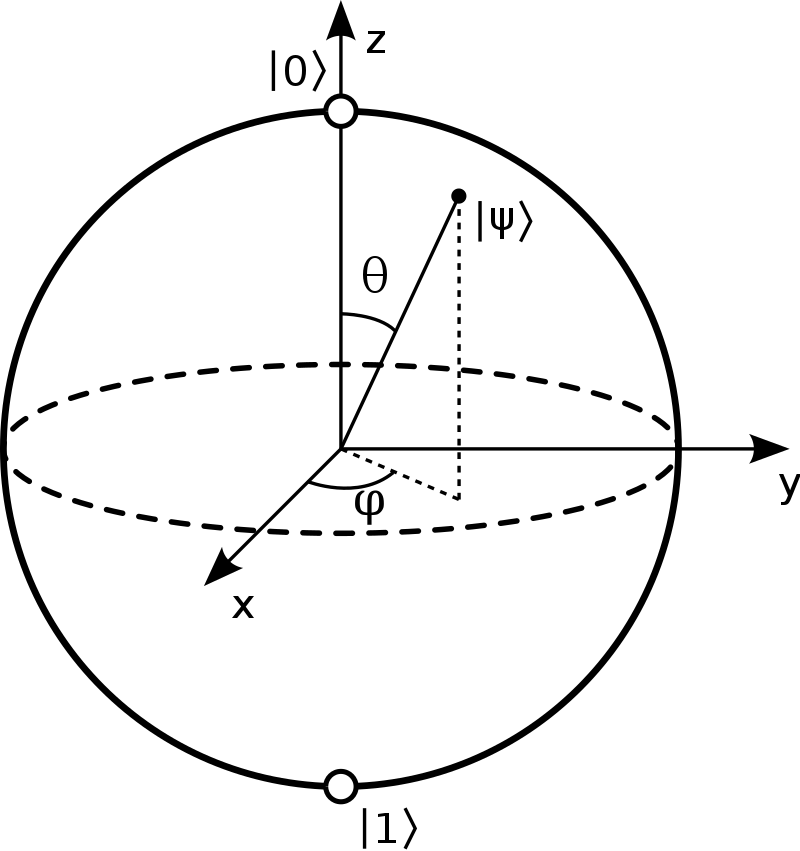
\includegraphics[width=0.5\textwidth]{Pictures/bloch_sphere.png}
% \vspace{0.3cm}\\
% Wikimedia Commons\cite{blochPicture}
% \end{center}
\end{titlepage}

\pagebreak
\tableofcontents
% Remove page number from contents page
\addtocontents{toc}{\protect\thispagestyle{empty}}
\pagenumbering{gobble}
\pagebreak

% Set headers
\pagestyle{fancy}
\pagenumbering{arabic}
\fancyhead{}
\fancyhead[L]{\leftmark}
\fancyhead[R]{\thepage}
\fancyfoot{}


\section{General Introduction to Quantum Computing}
Quantum computing is a type of computing that uses quantum mechanical phenomena to process information. Whereas classical computers use binary digits (\textit{bits}) to represent information as either $0$ or $1$, a quantum computer uses quantum bits (\emph{qubits}), which are quantum superpositions of two independent states: $\ket{0}$ and $\ket{1}$.\cite{candela} These qubit states can then be combined in the usual way via tensor product to represent multi-qubit systems. For example, a two-qubit system with the first qubit in state $\ket{0}$ and the second qubit in state $\ket{1}$ is denoted $\ket{01}$, which is formally given by the tensor product:\cite{nielsenChuang}
\begin{equation}
    \ket{01}\equiv\ket0\ket1\equiv\ket{0}\otimes\ket{1}
\end{equation}
Combinations of multiple qubits then introduces the property of \emph{entanglement}. This is a phenomenon whereby the properties of two or more particles/systems are correlated in some way, no matter how far apart they are in space.\cite{griffiths} For example, consider the following two-qubit state:
\begin{equation}
\frac{1}{\sqrt2}\left(\ket{01}-\ket{10}\right)
\end{equation}
This state corresponds to a $50\%$ probability of measuring the first qubit to be $0$ and the second equal to $1$, and a $50\%$ probability of measuring the opposite pairing. This indicates that just by measuring the state of one qubit you could instantly know the outcome of measuring the other. Hence measurements of the two qubits are statistically correlated with each other, and thus they are \emph{entangled}.\cite{griffiths} For a more formal definition, an entangled state $\ket{\psi}$ of a composite system is one that cannot be written simply as the product of two or more state vectors from the individual systems that comprise it, i.e. $\ket{\psi}\neq\ket{A}\otimes\ket{B}$.\cite{griffiths} This ability for qubits to become entangled is wholly unique to quantum computers. In a classical computer, the state of each bit is completely independent of all other bits and does not exist in any form of superposition.\\
\\
These quantum mechanical properties of superposition and entanglement allow quantum computers to perform certain types of calculations much faster than classical computers. For example, in some types of optimization problems, quantum computers can search all possible solutions in parallel by using entanglement to explore all possible combinations of values at the same time.\cite{candela} This can lead to a quadratic speedup over classical computers, which would have to search through each possible solution one at a time. Entanglement also plays a very important role in \textit{quantum cryptography}, where it can be used to securely transmit information over long distances. By entangling two particles and then sending them to separate locations, it is possible to create a secret key that can be used to encrypt and decrypt messages.\cite{quantumcrypt} Any attempt to intercept or measure the key would cause the entanglement to be broken, alerting the sender.\\
\\
However, quantum computing is still in its early stages and faces many challenges, such as the problem of maintaining the fragile state of qubits and controlling their interactions. Nevertheless, the potential of quantum computing is enormous and has many potential applications. In this paper we will explore two of these applications: the first is the use of that \textbf{Grover's algorithm} to search through an unstructured database. Classical linear search algorithms do not scale well for searching through large databases, but Grover's algorithm exploits quantum superposition to search through the entire database simultaneously.\cite{grover} The second will explore \textbf{Shor's algorithm} to decrypt a small scale version of RSA encryption. RSA encryption exploits the inability of classical computers to factorise large semiprime numbers efficiently,\cite{RSA} but Shor's algorithm can factorise large semiprimes in polylogarithmic time.\cite{Shors_algorithm}

\subsection{States, Operators and Quantum Circuits}
Just like a classical circuit, a quantum circuit is composed of a certain number of bits (or in this case, qubits), logic gates, and measurements. Quantum logic gates are a fundamental concept in quantum computing as they are used to implement quantum algorithms and perform quantum computations. However, there is a catch: \textbf{quantum gates must always be reversible.}\cite{nielsenChuang} Most classical logic gates are not reversible, meaning you cannot always recover the two input bits from the output bit. For example: if an AND gate gave an output $0$, then there is no way to know if the initial input was $00$, $01$, or $10$. In quantum mechanics it follows from the Schrodinger equation that quantum states always evolve in time via unitary transformations.\cite{griffiths} Hence all quantum gates must be unitary operators. Since all unitary operators have inverses by definition, this means all quantum gates must be reversible.\\
\\
Just like classical circuits, quantum circuits can be represented as a directed acyclic graph, where each node represents a quantum gate and the edges represent the flow of information between gates.
\begin{figure}[H]
\centering
\begin{subfigure}[t]{0.5\textwidth}
\centering
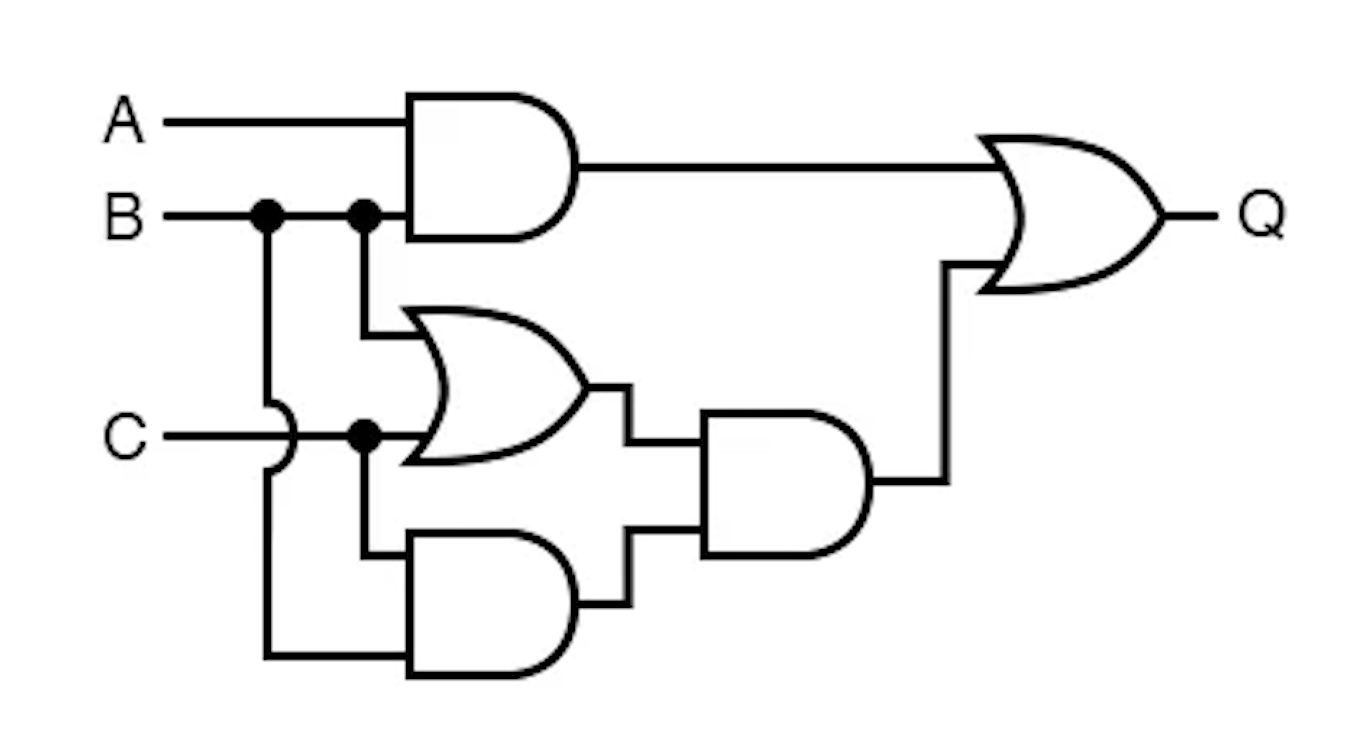
\includegraphics[width=0.7\linewidth]{Pictures/logicgates.png}
\caption{Classical}
\label{fig:circuitsub1}
\end{subfigure}%
\begin{subfigure}[t]{0.5\textwidth}
\centering
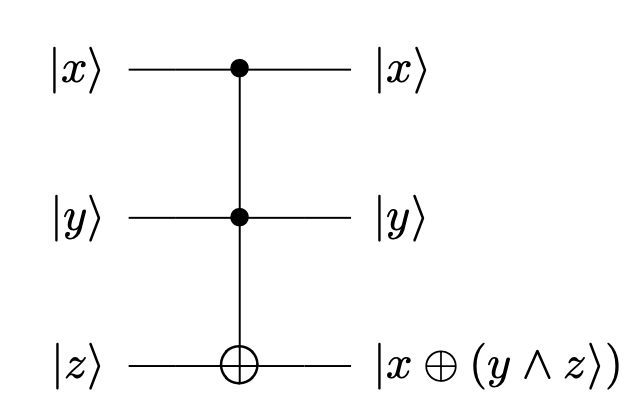
\includegraphics[width=0.7\linewidth]{Pictures/quantumcirc.png}
\caption{Quantum}
\label{fig:circuitsub2}
\end{subfigure}
\caption{(Left) Example classical circuit diagram composed of a series of logic gates. The $A$, $B$ and $C$ binary input signals are assumed to be provided from switches, sensors, or perhaps other gate circuits.\cite{circuitbook}\\(Right) Example quantum circuit diagram composed of \emph{quantum} logic gates. In this diagram we observe the so-called Quantum Toffoli Gate (CCNOT), which is defined for 3 qubits.\cite{exquantumcirc}}
\label{fig:circuit_examples}
\end{figure}

In a quantum circuit, the output of a computation is obtained by performing a measurement on the qubits, causing them to ``collapse'' into definite classical states (i.e. a classical bitstring). It is important to note that once a measurement is made, the original quantum state is lost and any subsequent measurements of the same qubits will only yield the same combination of classical bits.\\
\\
If we have a system $A$ with orthonormal basis $\ket{k}$ with $k=1,2,...,N_A$, and a system $B$ with orthonormal basis $\ket{m}$ with $m=1,2,...,N_B$, a joint state of these systems is be expressed as\cite{griffiths}
\begin{equation}
\ket{\psi}=\sum_{k,m}c_{k,m}\ket{km}\end{equation}
and an operator $\hat{F}$ acting on the state is written as
\begin{equation}\hat{F} = \sum_{k,m,l,n}F_{k,m,l,n}\ket{km}\bra{ln}\end{equation}
where $F_{k,m,l,n}=\bra{km}\hat F\ket{ln}$.\\
\\
Quantum gates operate on qubits by manipulating their superposition states. There are several different types of quantum gates that can be used in quantum circuits, including unary (single-qubit) gates, binary (two-qubit) gates and other multi-qubit gates. Unary gates are used to perform rotations and phase shifts on individual qubits, while multi-qubit gates are used to perform operations that entangle multiple qubits together. For example, the Hadamard gate, which acts on a single qubit, is a quantum gate that can be used to place a classical bit into a $50:50$ superposition state.\cite{nielsenChuang}
\begin{equation} \hat{H}=\frac{1}{\sqrt2} \begin{pmatrix}
1 & 1 \\
1 & -1\\
\end{pmatrix}\end{equation}
The CNOT (controlled-NOT) gate is a two-qubit gate that can be used to entangle two qubits
\begin{equation} CNOT= \begin{pmatrix}
1 & 0 & 0 & 0 \\
0 & 1 & 0 & 0\\
0 & 0 & 0 & 1\\
0 & 0 & 1 & 0\\
\end{pmatrix}\end{equation}
\\
These gates (as well as other more complex ones) will be used throughout this report. A table of commonly used quantum logic gates and their corresponding circuit symbols is located in the \hyperref[section:appendix]{Appendix.}

\subsection{Simulation of Quantum Circuits}\label{section:simulation}
To summarise, any quantum circuit consists of an initial state vector, a series of quantum gate applications and then a measurement at the end. A simulated qubit state vector can therefore be stored simply as a linear array and quantum gates can be stored as matrices. There are a vast number of matrix computing libraries that can handle this and for the purpose of this project NumPy\cite{python,numpy} was used. Once this is done, any quantum logic circuit can be simulated by following a few key rules.

\subsubsection{Simulating quantum logic gates}
To mathematically describe applying a quantum logic gate to a qubit state vector, we simply multiply the state vector by the gate's matrix. However, to apply a logic gate to a specific subset of the qubits we must also describe what occurs on all other qubits at the same time (which is essentially nothing). This is done through the use of tensor products.\cite{nielsenChuang} For example, consider a unary (single-qubit) gate $\hat A$ in a 2-qubit system. The action of $\hat A$ on qubit 1 is $\hat A\otimes I$ and on qubit 2 it is $I\otimes\hat A$, where $I$ is the 2-D identity matrix. Similarly, the circuit
\begin{center}
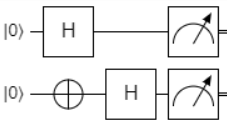
\includegraphics[width=0.25\textwidth]{Pictures/tiny-circuit.png}
\end{center}
corresponds to the the matrix multiplication $(I\otimes H)(H\otimes\sigma_x)\ket{00}$, followed by a measurement of the state vector.

For a binary (or larger) gate, the process of applying the gate to a subset of the qubits is a little more complicated. Consider the CNOT gate mentioned previously for a 3 qubit system. Whilst it is possible to apply this gate to adjacent qubits, it is also possible to apply them to non-adjacent qubits.
\begin{figure}[H]
    \centering
    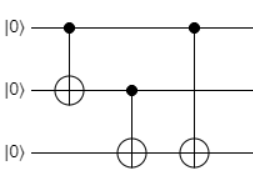
\includegraphics[width=0.3\textwidth]{Pictures/cnot-circuit.png}
    \caption{A quantum circuit built out of three CNOT gates. A CNOT gate is applied to qubits 1 and 2, then to qubits 2 and 3, then finally to qubits 1 and 3.}
    \label{fig:cnot_circuit1}
\end{figure}

In Figure \ref{fig:cnot_circuit1}, there are three binary quantum gates in the circuit, specifically CNOT gates. The first gate is applied to the first and second qubits and is hence equivalent to $\text{CNOT}(1,2)\otimes I$. The second gate is applied to the second and third qubits and is hence equivalent to $I\otimes\text{CNOT}(2,3)$. The third gate is applied to the first and third qubits and is not as simple to compute. There are multiple ways to get around this problem, but the solution used in this project was to use SWAP gates. As the name suggests, these can be used to swap the states of two qubits.\cite{nielsenChuang,candela}
\begin{equation}
\text{SWAP}=\begin{pmatrix}
1&0&0&0\\
0&0&1&0\\
0&1&0&0\\
0&0&0&1
\end{pmatrix}
\end{equation}
Using these SWAP gates, the circuit can be adjusted so that all binary gates are applied solely to adjacent qubits.
\begin{figure}[H]
    \centering
    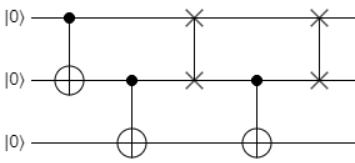
\includegraphics[width=0.4\textwidth]{Pictures/cnot-circuit-swap.png}
    \caption{An adjusted form of the circuit in Figure \ref{fig:cnot_circuit1}. By swapping qubits 1 and 2, it is possible to perform a logical operation which is completely equivalent to applying the CNOT gate to 1 and 3 without having to work with non-adjacent quantum gates.}
    \label{fig:cnot_circuit2}
\end{figure}
This method of using SWAP gates can then be extended trivially to even larger multi-qubit gates and larger qubit registers, so it is immensely effective. However, the downside of using this method is that for any multi-qubit gate the number of required matrix multiplications to compute it increases by \emph{at least} 2, if not more depending on how far apart the qubits are. This therefore increases the overall number of computations the classical computer needs to perform to simulate the quantum circuit.

\subsubsection{Simulating measurement}
To obtain the actual result from the quantum computation, the state vector must then be measured. For a physical quantum computer this of course means the actual qubits are measured using physical apparatus and the result is then a combination of classical bits. However, for a simulation it is not quite so simple, as we are instead performing mathematical manipulations on vectors in a Hilbert Space.

To simulate measurement, we instead use the fact that the state vector is itself a probability distribution. For a qubit state
\begin{equation}
\ket\psi=\sum_{n}a_n\ket{n}=a_{0}\ket{0}+a_{1}\ket{1}+\dots
\end{equation}
the probability of measuring the classical binary number $n$ is $p_n=|a_n|^2=a_n^*a_n$.\cite{griffiths} Using a random number generator it is possible to then simulate measuring a qubit state vector $\ket\psi$ via the following algorithm:\cite{candela} 
\begin{enumerate}
    \item Uniformly generate a random number $0\leq r\leq1$.
    \item Set some variable $q=0$.
    \item For each component $\psi_i$ in the state vector (starting from $\psi_0$) increase $q$ by $|\psi_i|^2$. If $q>r$ then the result of the measurement is $\ket i$. Otherwise, repeat this step for the next component in $\ket\psi$.
\end{enumerate}
This algorithm reproduces measurements consistent with the probability distribution described by $\ket\psi$. It is important to note that once the measurement has been performed, the state vector will collapse into the result of that measurement.\cite{griffiths} This means any further measurements of that state vector cannot yield a different result; once the quantum computation is done any result is final. To get a different result the entire quantum algorithm must be re-run.

\subsubsection{Hardware Limitations}
Since the simulated qubits and quantum gates need to be stored in the classical computer's memory, the scope of the project was limited by the hardware available to us. Each additional qubit causes the number of dimensions in the overall Hilbert space to double, meaning the memory required by the simulation increases exponentially with the number of qubits. It was found that the maximum number of qubits we could simulate on the hardware available was $n=14$ before running out of memory. However, the time taken to perform quantum logic on 14 qubits was prohibitively long, as each quantum gate would have $2^{28}$ elements. Thus all simulation was limited to a maximum of $n=13$ qubits.

\subsection{Simulation of Quantum Error}\label{section:error_intro}
The discussion of quantum computing thus far has remained very idealised and has assumed that all the qubit manipulations of qubits remain perfect and noise-free. Of course, in a real quantum computer this would hardly be the case. Quantum logic gates in a real quantum computer must be built out of physical components and will contribute random errors that will directly influence the overall state of the qubits.\cite{nielsenChuang} A good simulation of any quantum algorithm should then necessarily simulate this quantum error within its circuit model.

There are two obvious approaches to implement error into our simulation scheme. The first seems quite simple: when defining the matrices used for the quantum logic gates, randomly change some of the elements in these matrices so that they do not have the desired outcome (e.g. randomly change some element from 1 to -1 in some given matrix). However, there are immediate issues with this approach. The first issue is that this is not a particularly general method. There may be other sources of error in a real circuit (e.g. an error in the qubit itself) which would be very difficult for this ``element-changing'' scheme to model. A second, more fundamental issue is that randomly changing elements in quantum gates may turn them non-unitary. Any errors that occur in the system are caused by physical effects and, as discussed earlier, any change in the state of a quantum system must be described by a unitary operator, even these errors. This could be avoided by requiring the elements are changed in such a way to preserve unitarity, but implementing this would likely be a non-trivial task for such an already flawed method. Thus, a different approach was taken to simulating error.

A little context is required. Although qubits are superpositions of two states, their components are complex. This means any single qubit state is described by four real numbers. The requirement of unit length means one of these components is not independent of the other three. In other words, every qubit state vector is equivalent to a 3-D real vector of unit length. The set of all possible qubit states may therefore be visualised as a unit sphere, which is known as the \emph{Bloch Sphere.}\cite{nielsenChuang}
\begin{figure}[H]
    \centering
    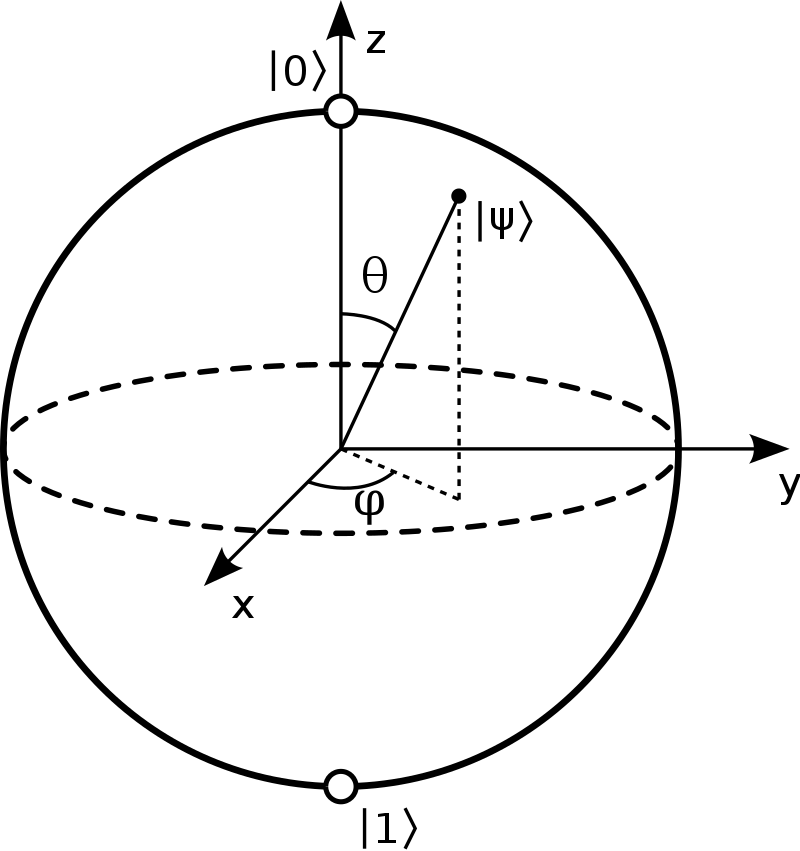
\includegraphics[width=0.25\textwidth]{Pictures/bloch_sphere.png}
    \caption{The Bloch Sphere. Any qubit state $\ket{\psi}$ may be represented as a real 3D vector lying on a unit sphere. The angles $\theta,\phi$ are spherical coordinate angles used to describe the location of the state on this unit sphere. Figure taken from Wikimedia Commons.\cite{blochPicture}}
    \label{fig:bloch_sphere}
\end{figure}
The point here is that any unary gate (i.e. single qubit gate) therefore corresponds to a rotation of the Bloch Sphere.\footnote{This is an example of the homomorphic relationship between $SO(3)$ (the 3-D rotation group) and $SU(2)$ (the 2-D unitary matrix group with positive determinant).\cite{chenGroup} Technically speaking there could also be unary gates with negative determinant that are hence not described by these rotations. However, in practice a negative determinant corresponds to multiplying the entire state vector by a global phase factor, which does not affect the final outcome of the circuit. Hence we can consider all unary gates to be $SU(2)$ operators.} Thus we can simulate error in a quantum circuit by generating randomised (small-angle) 3-D rotations that occur at random points in the circuit.

For rotation by an angle $\theta$ about an axis aligned with a unit vector $\mathbf{\hat n}$, the corresponding 2-D unitary matrix is given by:\cite{nielsenChuang,chenGroup}
\begin{equation}
R(\theta,\hat n)=e^{-i\frac{\theta}{2}\mathbf\sigma\cdot\mathbf{\hat n}}=\cos\frac{\theta}{2}I-i\sin\frac{\theta}{2}\left(n_x\sigma_x+n_y\sigma_y+n_z\sigma_z\right)
\end{equation}
where $I$ is the 2-D identity matrix and $\sigma_x,\sigma_y,\sigma_z$ are the Pauli matrices. Between every application of a quantum logic gate we then run the following algorithm:
\begin{enumerate}
    \item Select an ``error probability'' $0\leq p_e\leq1$ and an ``error size'' $0\leq\Omega\leq1$ at the start of the simulation. The same values of $p_e,\Omega$ are used throughout the entire simulation.
    \item For each qubit, uniformly generate a random real number $\epsilon$ between $0$ and $1$ inclusive. If $\epsilon\leq p_e$ then this qubit is ``marked'' to experience an error.
    \item For each marked qubit $i$:
    \begin{enumerate}
        \item Generate a random real number $\omega$ such that $0\leq\omega\leq\Omega$. The rotation angle for the error is then $\theta=4\pi\omega$.
        \item Uniformly generate 3 random floating point numbers between $0$ and $1$ and inclusive. For each of these numbers choose to flip their sign from positive to negative with a 50\% probability. Then store these numbers as the components of a vector and normalise them. This is the rotation axis vector $\mathbf{\hat n}$.
        \item Compute the ``error gate'' $E_i=\cos\frac{\theta}{2}I-i\sin\frac{\theta}{2}\left(n_x\sigma_x+n_y\sigma_y+n_z\sigma_z\right)$.
    \end{enumerate}
    \item For all other unmarked qubits $i$, set $E_i=I$
    \item Compute the overall error gate $E=\bigotimes_{i}E_i=I\otimes E_2\otimes E_3\otimes I\dots$, with error gates appearing at their appropriate positions in the tensor product.
    \item Insert the error gate into the circuit.
\end{enumerate}
Ideally the error size should be chosen to be a small number (e.g. $\Omega=10\%=0.1$) to simulate quantum error. However, it is important to note that the ``magnitude'' of the errors is not necessarily proportional to the magnitude of $\Omega$ because $\cos$ and $\sin$ are periodic functions.

The advantages of this approach are that it preserves the unitary of the overall circuit, it is much more general than the first approach and it is relatively easy to scale to different numbers of qubits (actual computation time and memory requirements notwithstanding). However, the fact the error gates are built out of tensor products of $SU(2)$ gates instead of using $SU(2^n)$ gates means they are completely separable and thus this algorithm cannot simulate accidental entanglement of qubits. However, that approach would require computing the generators of $SU(2^n)$ and using those to compute the error gates. This would be much harder to implement and more computationally expensive for what at small scales is essentially only a minor improvement on this algorithm.


\pagebreak
\section{Grover's Algorithm and Exoplanet Habitability}\label{section:groverproject}
\subsection{Grover's Algorithm}
Consider an \emph{unstructured} database with $N$ different entries, from which we would like to find one specific element. To find it, a classical computer would have to look through each one in order until the target is found. If we are lucky, this target would be first item in our database. However if the target were located at the end of the list, then our classical computer would have to look at all $N$ entries to find it. In general, the classical computer would have to look at $N/2$ entries on average. This means unstructured linear search has a \emph{time complexity} of order $O(N)$ (i.e. as the number of inputs $N$ increases, the number of required steps in the search algorithm increases at the same rate).\cite{candela} Ultimately, this means that although it would not take much time to search through a small database, it becomes much slower once we start working with a much larger database.

Grover's algorithm attempts to solve this problem by providing a quadratic speedup (i.e. time complexity $O(\sqrt N)$) over such classical search algorithms by exploiting quantum superposition to effectively search the entire database simultaneously.\cite{candela,grover} This quadratic speedup is a large decrease in computation time if $N$ is very large. First, this algorithm must put convert the database search into the form of a \textit{``quantum oracle''}. This is a quantum logic gate that accepts a qubit state of index registers and returns the corresponding quantum superposition of ``answers.''\cite{candela} If the oracle is given one of the $N-1$ wrong database entry states, it must return that state unchanged. However, if the qubit state corresponds to the position of the target element, it returns that state multiplied by $-1$. We do this by setting the oracle to be the identity matrix, except that it has a $-1$ on the diagonal element corresponding to the correct entry.

More formally, let $f(x)$ be some function of a combination of classical bits and let $x_0$ be a target element. We specify that $f(x=x_0)=1$ and $f(x\neq x_0)=0$. This is called an ``oracle function'' and it corresponds to asking the question ``is target $x_0$ located at index $x$ in the database?'' The corresponding quantum oracle $\hat O$ is then given by
\begin{equation}
\hat O\ket x = (-1)^{f(x)}\ket x
\end{equation}
For example (using a 3-qubit register for simplicity), if the target entry is located at index $110$, then the quantum oracle would be\footnote{At first glance, it seems it would make more sense to define the quantum oracle in a different way and set every element equal to $0$ except the diagonal corresponding to the target. However, such a matrix is not unitary and hence is not a valid quantum logic gate.}
\begin{equation} \hat{O}= \begin{pmatrix}
1 & 0 & 0 & 0 & 0 & 0 & 0 & 0 & 0\\
0 & 1 & 0 & 0 & 0 & 0 & 0 & 0 & 0\\
0 & 0 & 1 & 0 & 0 & 0 & 0 & 0 & 0\\
0 & 0 & 0 & 1 & 0 & 0 & 0 & 0 & 0\\
0 & 0 & 0 & 0 & 1 & 0 & 0 & 0 & 0\\
0 & 0 & 0 & 0 & 0 & 1 & 0 & 0 & 0\\
0 & 0 & 0 & 0 & 0 & 0 & 1 & 0 & 0\\
0 & 0 & 0 & 0 & 0 & 0 & 0 & -1 & 0\\
0 & 0 & 0 & 0 & 0 & 0 & 0 & 0 & 1\\
\end{pmatrix}\end{equation}
The algorithm also requires an operator $\hat{J}$, which is just like the oracle, but with the -1 value in the first entry:\cite{candela}
\begin{equation}
\hat J = \hat I-2\ket{0}\bra{0}
\end{equation}

Now we have all the necessary elements to construct our circuit. First, all qubits are put in an equal superposition of all eight\footnote{The number of basis states on a system equals $2^N$ where $N$ is the number of qubits, since each qubit can exist in one of two possible states.} basis states. We do this by applying a first set of Hadamard gates, as shown in Figure 1, followed by the quantum oracle, which will ``ask all $2^N$ questions simultaneously'' and will change the sign of the component for the correct index.

We then apply a series of Hadamard gates again, followed by $\hat J$ and then another series of Hadamard gates (i.e. the matrix $\hat H^{\otimes n}\hat J\hat H^{\otimes n}$). This series of gates forms the \textit{Grover diffusion operator}, which is designed to convert the phase difference into a component-wise magnitude difference\cite{candela}, which we can measure. By successively applying the oracle and diffusion operator multiple times, the initial state will asymptotically approach the state corresponding to the target index. For $n$ qubits we only need to apply this pair of gates $O(\sqrt{2^n})$ times to have a high probability of success,\cite{grover,candela} which is much lower than the $O(2^n)$ a classical linear search would require.

\begin{figure}[H]
\centering
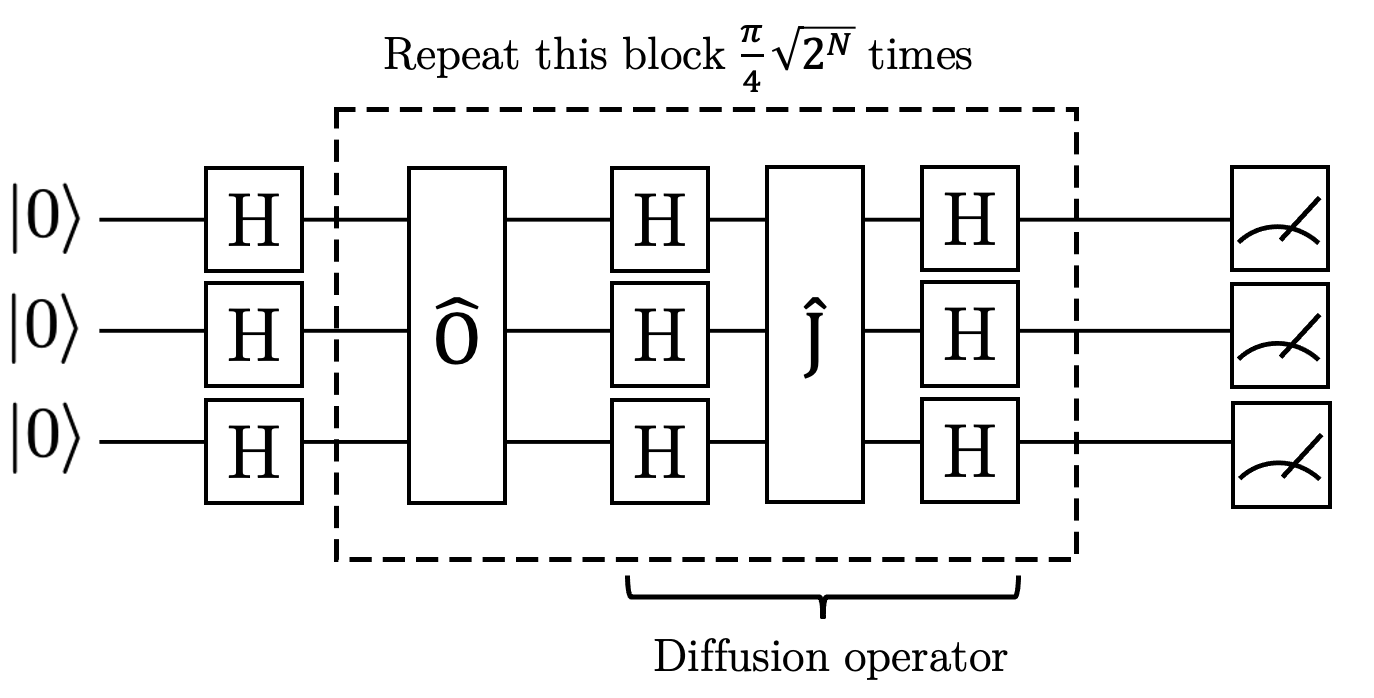
\includegraphics[width=0.6\textwidth]{Pictures/groversketch.png}
\caption{3-qubit quantum circuit diagram for Grover's algorithm}
\end{figure}

\subsection{Grover Adaptive Search (GAS) and the Durr-Hoyer Algorithm}\label{section:GAS}
Although Grover search is usually expressed as a simple search algorithm, the fact it is so efficient means it is well suited to optimising functions by ``searching'' for inputs that give optimal elements. These can be found via an extension of the algorithm known as Grover Adaptive Search (GAS), which makes use of multiple fast Grover searches to find successively ``better'' outputs.

More specifically, GAS is designed to find an input region that maximises/minimises a function $f:S\rightarrow\mathbbm R$ through successive Grover searches. There are multiple variants of the GAS algorithm,\cite{baritompa} however in this paper we will focus on a slight modification of the version first described by Durr and Hoyer.\cite{durrhoyer,baritompa} This variant of the algorithm works as follows:
\begin{enumerate}
    \item Select an element $X_0\in S$ at random, where $S$ is the input space. Set $Y_0=f(X_0)$. Call this the ``pivot.''
    \item Set $m=1$ and select a scaling factor $\lambda$. For the implementation in this project $\lambda=1.34$ as it is known to be a good scaling factor.\cite{baritompa}
    \item For $n=1,2,\dots$
    \begin{enumerate}
        \item Pick a random iteration count $r\in\mathbbm N$ between $0$ and $\lceil m \rceil$
        \item Define an oracle function $g(x)$ such that $g(x)=0$ if $f(x)<f(X_0)$ and $g(x)=1$ if $f(x)>f(X_0)$ (assuming we are searching for a maximum. If we are searching for a minimum the inequalities are flipped).
        \item Perform a Grover search of $r$ iterations on the set $S$ using this oracle function and measure the output. Call this $x$ and $y=f(x)$.
        \item If $y>Y_n$ (or $y<Y_n$ if we are searching for minima), then this is the ``new best element'' and so it is used as the new search pivot. Hence set $X_{n+1}=x$, $Y_{n+1}=y$. Otherwise, stick with the previous pivot and so set $X_{n+1}=X_n$, $Y_{n+1}=Y_n$.
        \item Repeat all of step 3 with a new maximum number of iterations $m'=\lambda m$ until a predefined termination condition is reached (this will depend on the specific optimisation problem).
    \end{enumerate}
\end{enumerate}

The advantage of this algorithm is that the oracle needs no information about the actual structure of the function to find the maximum/minimum.\cite{baritompa} Instead, these successive Grover searches simply cause the algorithm to take a targeted random walk through the input space to the optimum region.
\begin{figure}[H]
	\fbox{\begin{minipage}[c]{0.45\textwidth}
			\caption{A diagrammatic representation of a Grover Adaptive Search to find the element at the minimum distance from the circle's centre. The algorithm starts at a random point and then uses Grover searches to find random elements at successively lower distances from the centre, thereby taking a guided random walk to the optimal element where it ends.}
		\end{minipage}\hfill
		\begin{minipage}[c]{0.6\textwidth}
			\centering
			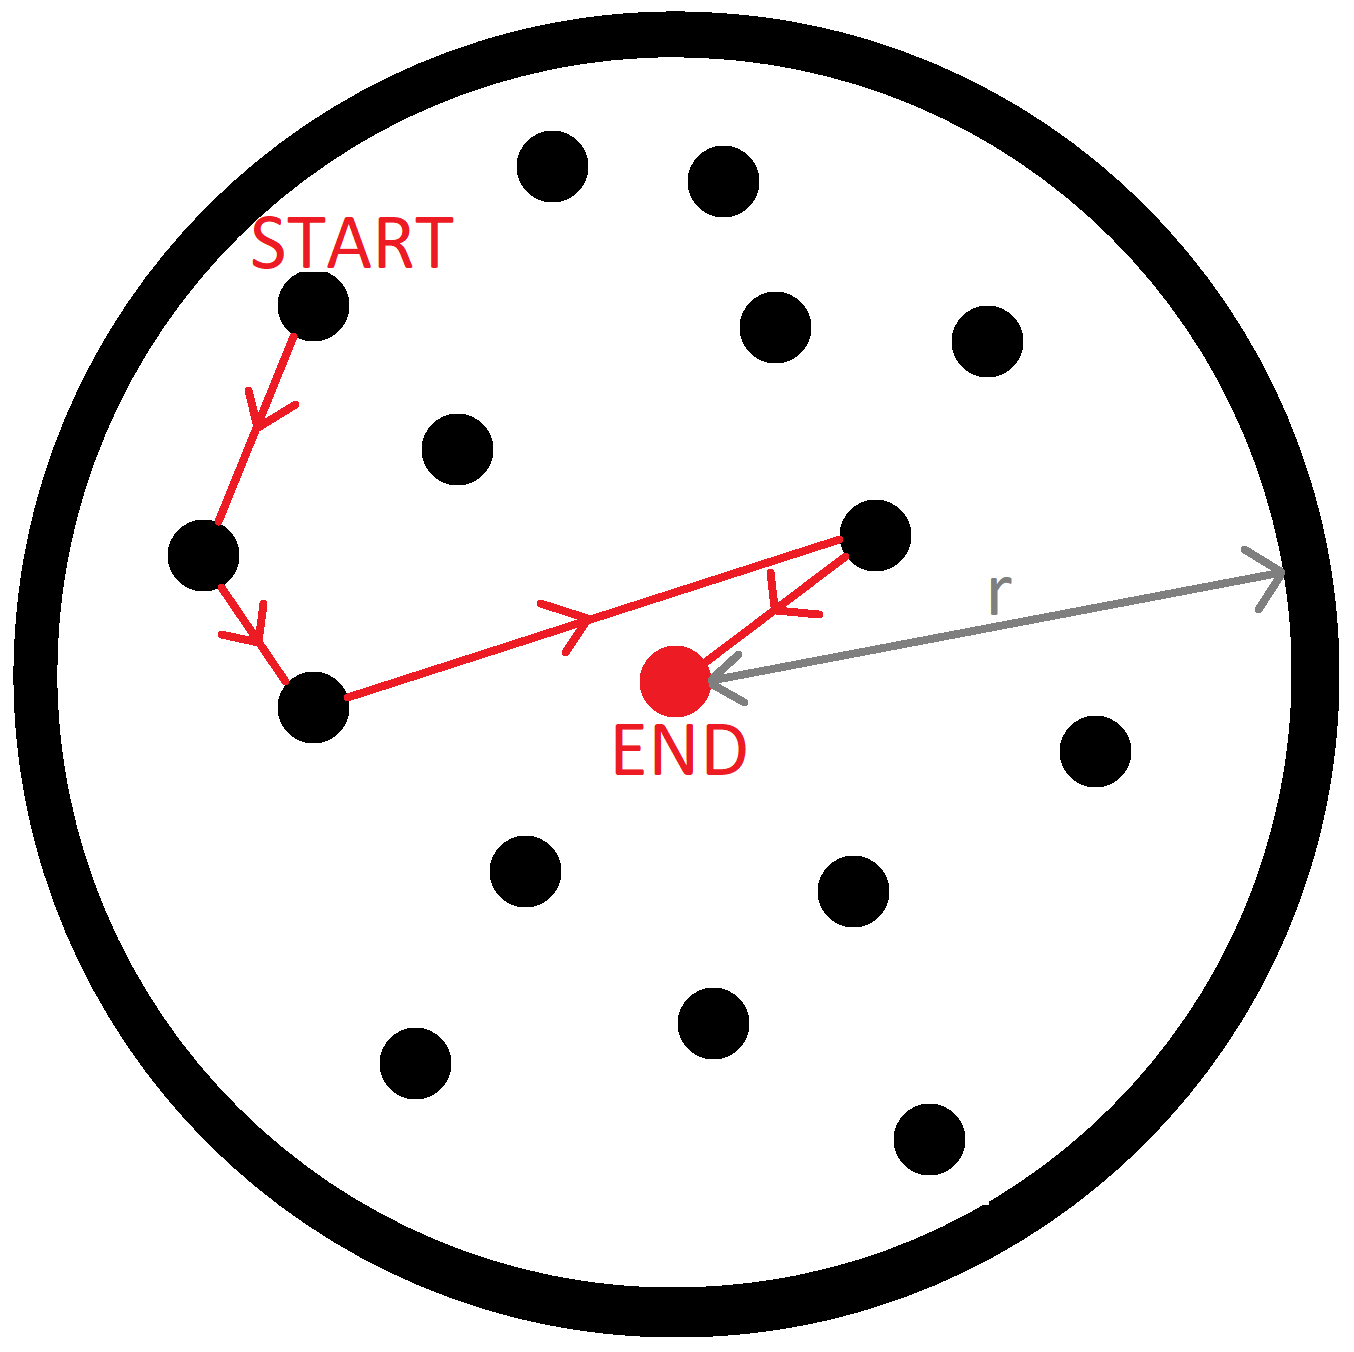
\includegraphics[width=0.55\textwidth]{Pictures/gas_diagram.png}
	\end{minipage}}
\end{figure}

\subsection{Finding Habitable Exoplanets in a Database}
\subsubsection{Exoplanet Habitability and the Earth Similarity Index}
The search for habitable planets has been a topic of interest in physics for many years, however, it is just recently that the investigation has intensified with the development of new technologies that allow us to detect and study planets outside our solar system, known as \textit{exoplanets}. Since the discovery of the first exoplanet in 1992\cite{exoplanet} thousands of exoplanets have been detected and studied. In particular, physicists have been interested in identifying exoplanets that could potentially support life as we know it, by looking for planets with conditions similar to those on Earth. This is where the Earth Similarity Index (ESI) comes in.
The ESI is a measure of the similarity of an exoplanet to Earth in terms of its physical characteristics such as its radius, surface temperature, and density.\cite{ESIpaper} This parameter ranges from $0$ to $1$, with $1$ being the most similar, i.e., the Earth itself.  We can calculate the ESI of a planet $j$ using the following formula:

\begin{equation}\label{eqn:ESI}
ESI_j=\prod^n_{i=1}{\left(1-\frac{x_{i,j}-x_{i,\bigoplus}}{x_{i,j}+x_{i,\bigoplus}}\right)^{w_i/n}}
\end{equation}
\\
\begin{center}
\begin{tabular}{||c|c|c|c||}
\hline
$i$ & \textbf{Parameter} & \textbf{Earth value} $x_{i,\bigoplus}$ & \textbf{Weight} $w_i$ \\
\hline
1 & Radius  & 1.0  & 0.57 \\
\hline
2 & Density  & 1.0 & 1.07 \\
\hline
3 & Escape velocity  & 1.0 & 0.7 \\
\hline
4 & Surface temperature & 288K & 5.58 \\
\hline
\end{tabular}
\end{center} 

Using the Extrasolar Planets Encyclopaedia\cite{EPE} we extracted a database with over 5300 exoplanets, from which we needed the entries with a value for mass, radius, and temperature. From this database, only 745 exoplanets had all those three values filled in, so we created a new trimmed database with solely those exoplanets, and calculated their corresponding ESI.\footnote{See Appendix \ref{appendix:ESI}.}

\begin{figure}[H]
\centering
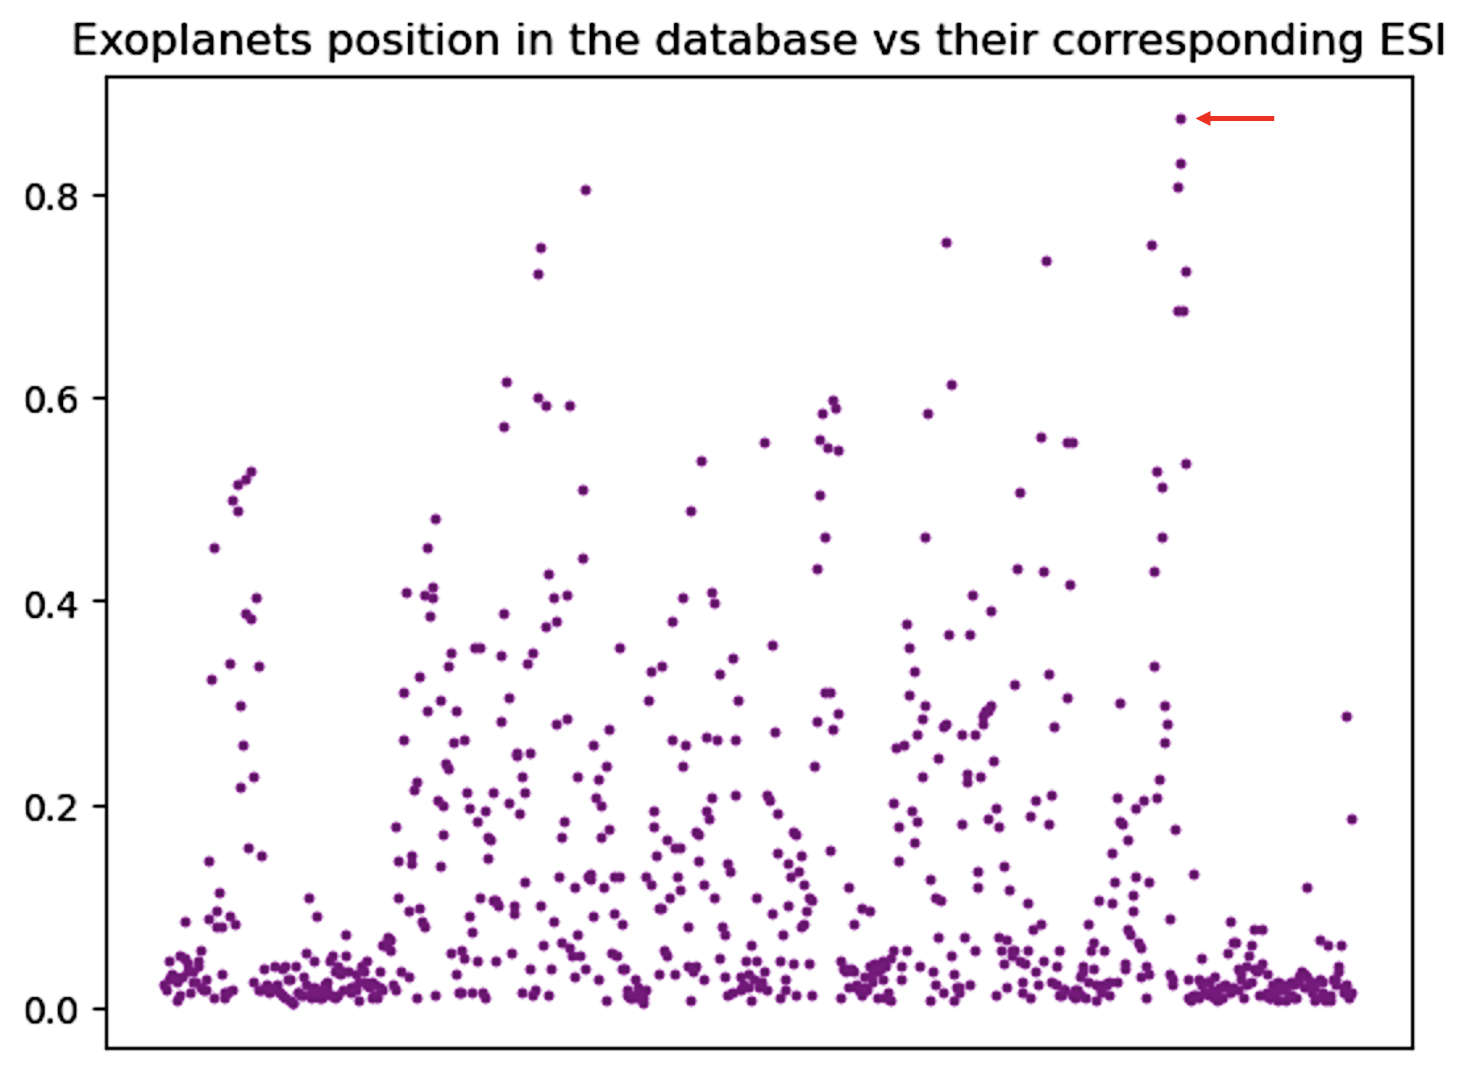
\includegraphics[width=0.6\textwidth]{Pictures/esiplot.png}
\caption{Values obtained for the Earth Similarity Indices of each exoplanet on the trimmed database. The position of each planet in the x-axis corresponds to its position on the new database. Planets are sorted alphabetically, \emph{not} by ESI. The value closest to 1 is highlighted with an arrow.}
\label{fig:ESIplot}
\end{figure}

The exoplanet with the closest ESI value is \textit{Trappist 1-D}, highlighted with an arrow on Figure 7. It has an ESI of approximately $0.8731$, as calculated using Equation \ref{eqn:ESI}.

\subsubsection{Applying GAS to the Database}\label{sec:GASonESI}
Although it was trivial to find the element with the highest ESI by inspection of Figure \ref{fig:ESIplot}, the aim is to implement GAS to search through the database to find this element. However, in subsection \ref{section:GAS} a crucial component was not discussed in depth: \emph{how to know when to stop}. If the algorithm is searching for an ESI in a certain range (which is what the Durr-Hoyer algorithm is originally designed for) then this is trivial: it terminates as soon as it finds an element in that range. However, it is not so trivial when searching for a single global maximum in the database.

To search for a global maximum, a new parameter known as the threshold $\mu$ was introduced. This was used in the following modification to the Durr-Hoyer algorithm:
\begin{enumerate}
    \item At the start of the program, we define a variable $f$ to count the number of ``failed'' Grover searches. Set $f=0$.
    \item After an individual Grover Search, the output of that search is compared with the ``pivot'' and it is then decided if the output of the Grover search is used as the new pivot, as discussed in step d of the Durr-Hoyer algorithm. If it is not chosen as the new pivot, increase $f$ by 1. If it is, reset $f$ to 0.
    \item Once $f=\mu$, terminate.
\end{enumerate}

The value of $\mu$ had to be appropriate to the size of the dataset: if it were too low the algorithm would be more likely to fail and if it were too high the algorithm would just perform unneccessary extra computation.

To find a good choice of $\mu$, the algorithm was ``trained'' on a different dataset of similar size. Since the ESI database contains 745 exoplanets, it had to be indexed by 10-bit integers. A database of $2^{10}$ elements was therefore generated with randomised elements between 1 and 800 inclusive and the first element was then set equal to 0 so that there was a well-defined global minimum. The Durr-Hoyer algorithm was then applied to this database for different values of the threshold for 10 trials of 100 shots to find the global minimum. Terminating on an element that was not the first element was deemed a failure. The number of fails was then counted to find the overall ``fail rate.''
\begin{center}
\begin{tabular}{||c|c|c||}
\hline
$\mu$ & Mean Fail Rate (\%) & Mean Fail Rate Uncertainty (\%)\\
\hline
1 & 99.90 & 0.30\\
2 & 93.60 & 2.29\\
3 & 73.40 & 2.58\\
4 & 44.60 & 6.70\\
5 & 26.60 & 5.28\\
6 & 16.40 & 3.23\\
7 & 9.60 & 1.62\\
8 & 5.00 & 2.00\\
9 & 1.90 & 1.22\\
10 & 1.20 & 1.17\\
\hline
\end{tabular}
\end{center} 
It was deemed that a failure rate of 5\% was the maximum tolerance, so $\mu=9$ was chosen as the threshold for our implementation of the Durr-Hoyer algorithm.

Now having trained on the randomised database to select $\mu$, the Durr-Hoyer algorithm was then applied to the database of exoplanets and their ESIs to find the entry with the highest ESI.
\begin{figure}[H]
\centering
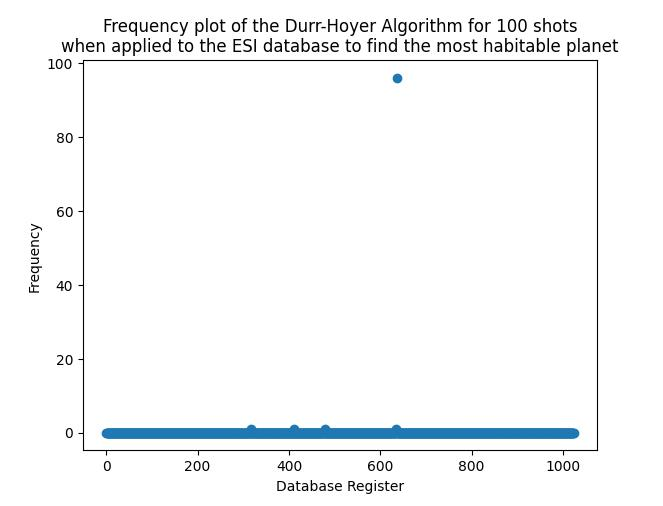
\includegraphics[width=0.6\textwidth]{Pictures/trappist.jpg}
\caption{Output of the Durr-Hoyer algorithm as applied to the exoplanet database for 100 shots. The most frequent result was the register $x=636$ in the database. Note that the x-axis exceeds 744 (the maximum register index) as the algorithm requires use of all 10 qubits, leading to 1024 possible outputs. This is not a problem as the search algorithm prevents these being actual measured outputs.}
\label{fig:GASfirstsearch}
\end{figure}

As seen in Figure \ref{fig:GASfirstsearch}, the most frequently obtained output of this algorithm was the index $x=636$, being located by 96\% of the shots. This corresponded to the position of the exoplanet \textit{Trappist 1-D} in the database as expected, confirming that the Durr-Hoyer algorithm worked correctly when applied to the database. However, this was without the inclusion of error modelling, as outlined in section \ref{section:error_intro}.

\subsection{Tests of Grover Search and the Durr-Hoyer Algorithm}
Figure \ref{fig:GASfirstsearch} is a good demonstration of the effectiveness of the Durr-Hoyer Algorithm in finding the global maximum in the ESI database, but it does not say much about the actual behavioural properties of the algorithm. For further tests of the algorithm we will use randomly generated databases instead. This opens the possibility of varying the number of qubits from 10, allowing for greater insight into the algorithm and also decreasing the computation time significantly if lower qubit counts are used.

\subsubsection{Searching for a range of values}
Instead of searching for a global maximum, it is also useful to search for a range of values in a database rather than a specific target. This means terminating the program once an element in the desired range is obtained, rather than using the ``termination threshold'' method outlined in section \ref{sec:GASonESI}.

The database now being searched through was randomly generated, containing values between 0 and 800 inclusive, except for the first element which is set to 801. This contained $2^n$ elements, where $n$ was the number of desired qubits (which can now be varied). The Durr-Hoyer algorithm was then implemented to find elements in this database greater than some minimum value $m$, which could vary between 0 and 800. It was expected that the algorithm's runtime would decrease when $m$ decreased. This is because a decrease in $m$ corresponds to a larger number of allowed search results, which would mean the algorithm terminates sooner. This was exactly the result observed.

\begin{figure}[H]
\centering
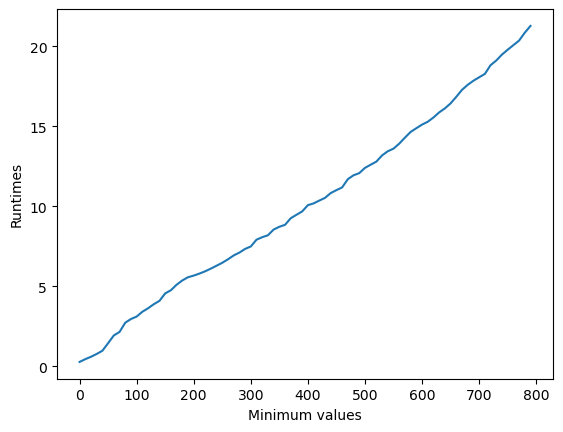
\includegraphics[width=0.65\textwidth]{Pictures/runtime2plot.png}
\caption{Relationship between the different minimum values $m$ and the time taken to run the simulation of the Durr-Hoyer algorithm for a 3-bit (8 element) database which is randomly generated.}
\label{fig:runtime2}
\end{figure}

In Figure \ref{fig:runtime2} we observe an approximately linear relationship between the minimum values and the overall runtimes. Since a larger minimum value corresponds to a smaller target region, this means the runtime is inversely proportional to the size of the target region, as hypothesised.

\subsubsection{Error Simulation}
Through the use of randomised small rotations of the qubit states, as explained in detail in section \ref{section:error_intro}, a simulation of qubit error was implemented which could be varied and tested for various noise levels.

The implementation of Grover's algorithm (not GAS) was then tested against this noise. Grover search was applied to a database indexed by 5 bits with the target index set to the first element. The error probability and the size of the errors were then both varied and the algorithm was tested over 20 trials of 100 shots.
\begin{figure}[H]
    \centering
    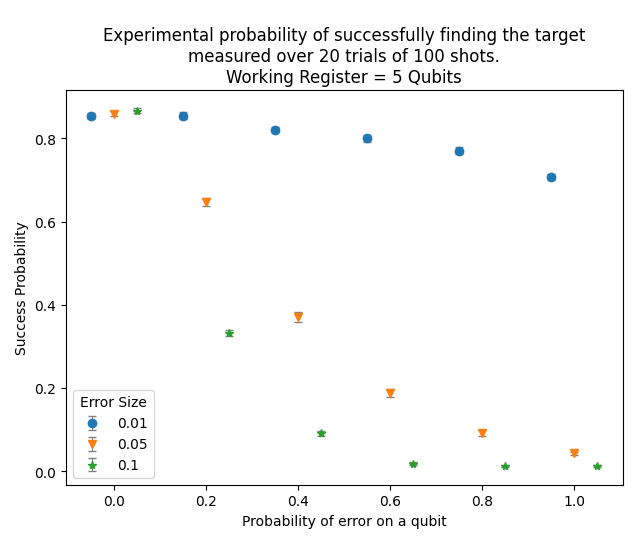
\includegraphics[width=0.8\textwidth]{Pictures/grover_errors.png}
    \caption{Probability of Grover's algorithm successfully locating the target element in the 5-bit database for different values of the error probability $p_e$ and the error size $\Omega$. It can be seen that a larger value of $\Omega$ directly correlates to a more rapid decay in the success probability over the range of error probabilities. Overall it is clear that quantum error has very adverse effects upon Grover's Algorithm.}
    \label{fig:grover_error}
\end{figure}

It can be seen in Figure \ref{fig:grover_error} that increases in both the error probability and the error size correlate directly to a decrease in the probability that Grover's Algorithm successfully locates the target. This is as expected, since the errors will lead to changes in the state of the qubit state vector that Grover's Algorithm cannot correct and the magnitude of said changes will depend on both how frequent and how large the errors are.

The error simulation was then incorporated into the implementation of the Durr-Hoyer Algorithm as it searched through the randomised database for a target range. We expected the algorithm to be stable against errors this time, since it would only terminate once in the target range. However, since it has been demonstrated that an increase in error causes Grover search to fail more often, an increase in runtime was expected for increasing error probabilities as the adaptive algorithm would have to compensate by performing more Grover searches. Again, this was exactly what was observed.

\begin{figure}[H]
\centering
\begin{subfigure}[t]{0.5\textwidth}
\centering
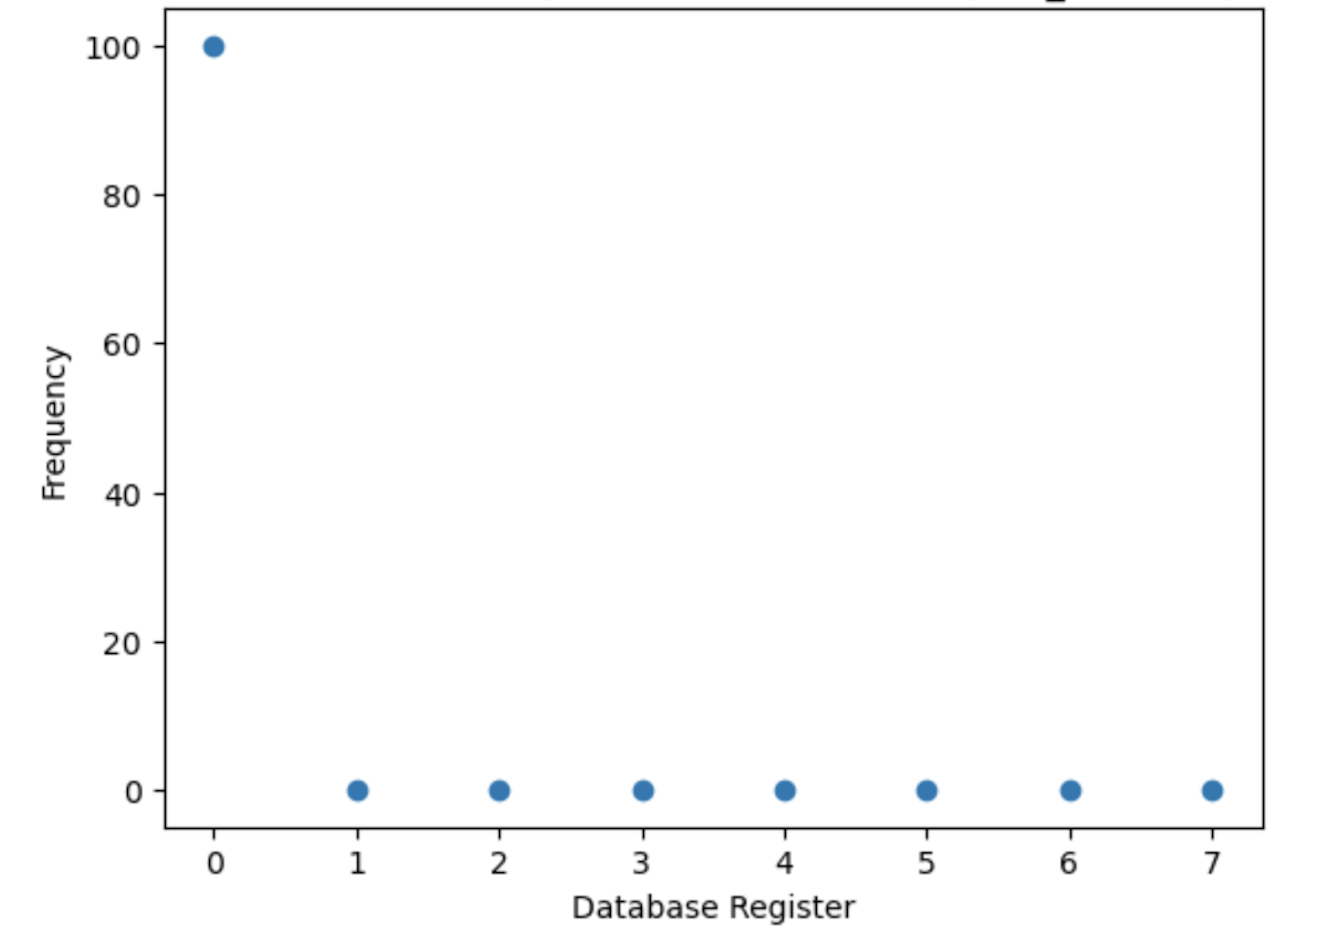
\includegraphics[width=\linewidth]{Pictures/errorp0.png}
\caption{Error probability = 0.}
\label{fig:errorp0}
\end{subfigure}%
\begin{subfigure}[t]{0.5\textwidth}
\centering
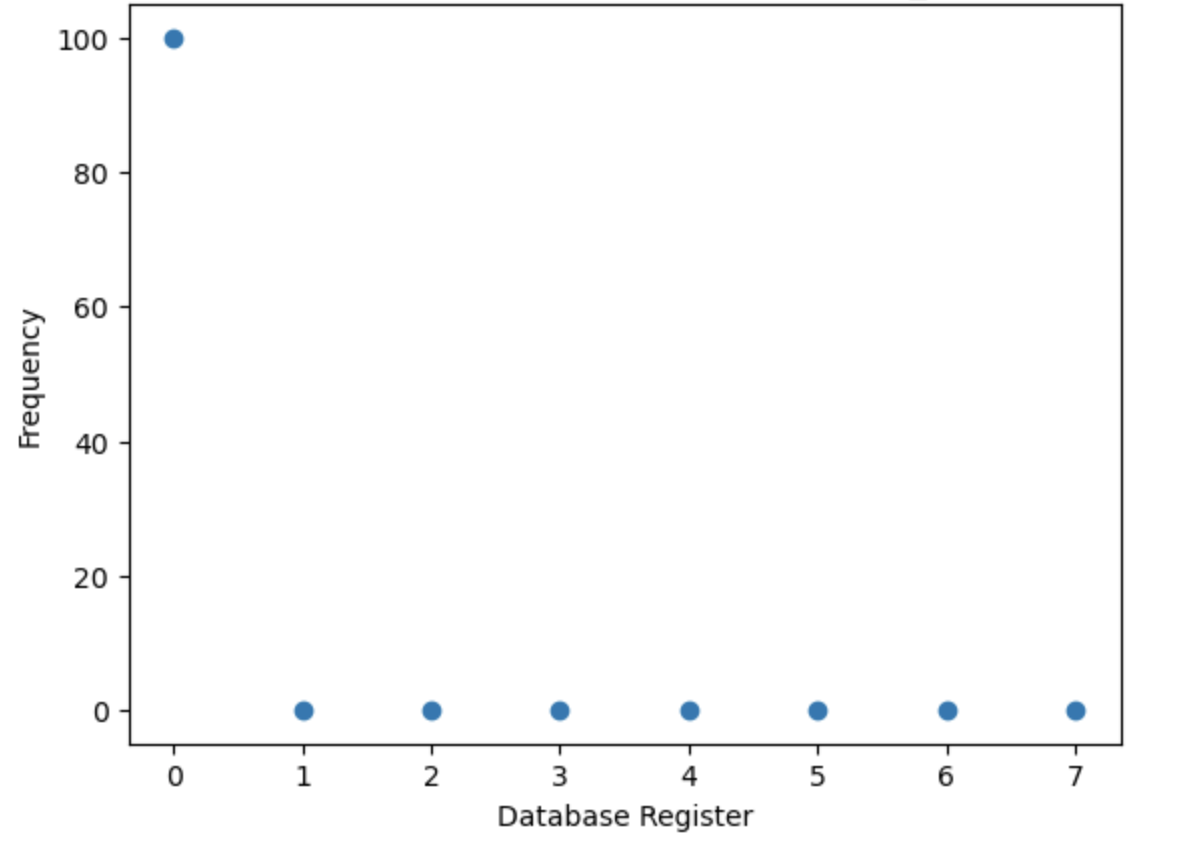
\includegraphics[width=\linewidth]{Pictures/errorp9.png}
\caption{ Error probability = 0.9.}
\label{fig:errorp9}
\end{subfigure}
\caption{Frequency plot of the Durr-Hoyer algorithm when applied to a randomised 3-bit (8 element) database. Minimum value = 800.}
\label{fig:durr_errors}
\end{figure}

\begin{figure}[H]
\centering
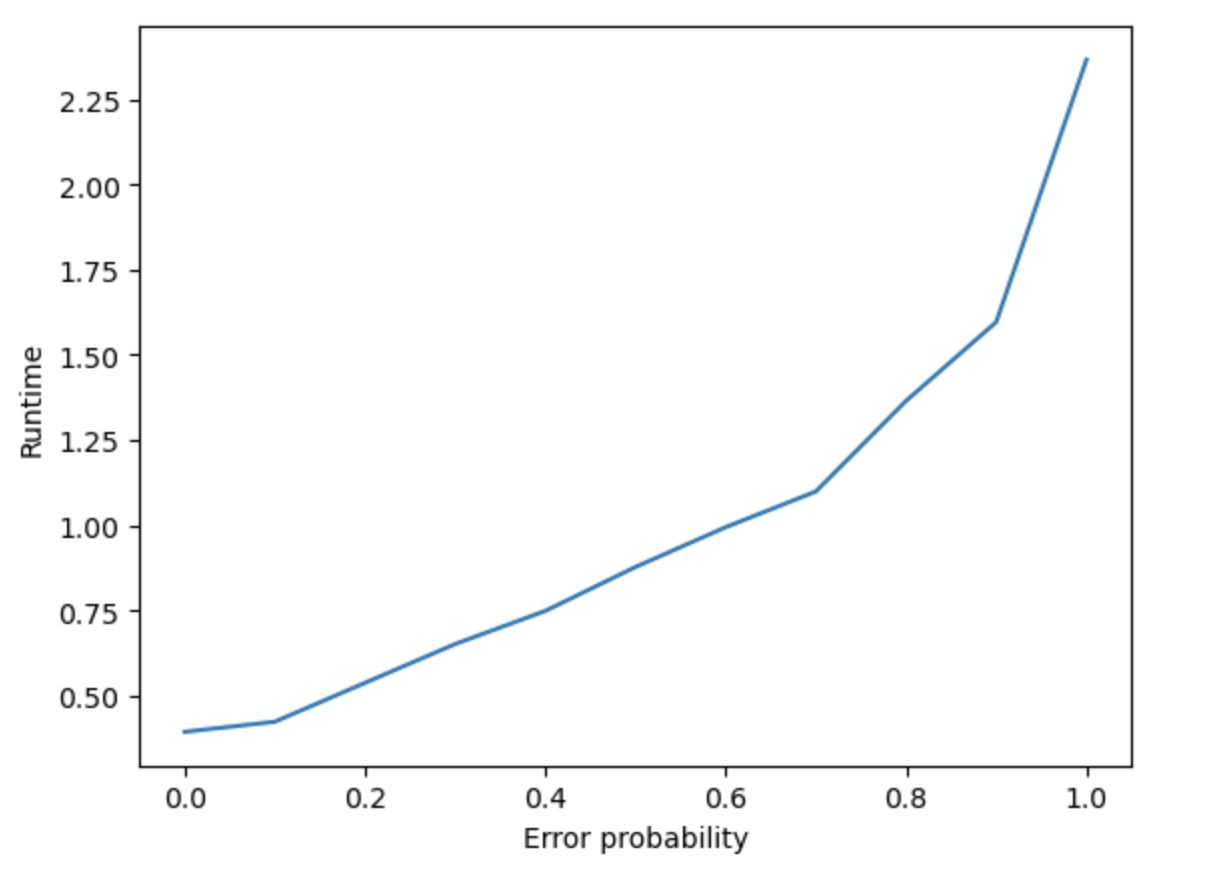
\includegraphics[width=0.8\textwidth]{Pictures/runtimeplot.png}
\caption{Relationship between different error probabilities and time taken to run the simulation of the Durr-Hoyer algorithm for a 3-bit (8 element) database which is randomly generated.}
\label{fig:runtimeplot}
\end{figure}

As expected, we observe in Figure \ref{fig:durr_errors} that the algorithm is stable against different error probabilities. This makes sense, since the algorithm only terminates once it finds a value in the given region. Instead, any increase in the error probability would rather affect the runtime of the program.\footnote{Further graphs like Figure \ref{fig:errorp0} and Figure \ref{fig:errorp9} for different values of error probabilities, as well as the different runtime values obtained to plot Figure \ref{fig:runtimeplot}, can be found in Appendix \ref{section:errorps}.}

As seen in Figure \ref{fig:runtimeplot}, the runtime is dependent on the error probabilities - an increase of the former implies an increase in the latter. We could also intuitively guess from Figure \ref{fig:runtimeplot} that the relationship between the increase of error probabilities and the algorithm's runtime is exponential. This would make sense, since an increase in the error probability would exponentially increase the number of error gates (since each insertion of an error gate is statistically independent, the probability of \emph{not} having a given number of error gates would exponentially decrease). However, much larger scale tests would be needed to verify this claim.

\subsection{Hardware Acceleration}
In general, running a simulation of Grover search on a classical computer is a slow process due to the large number of computations involved. The ESI database requires 10 qubits to search, which means the matrices describing each quantum gate in the circuit contain 1,048,576 elements. This is a large number of computations to perform and can only be done in a reasonable amount of time through the use of parallel computation (i.e. running an algorithm that performs multiple computations simultaneously through the use of multiple cores in a single processor). Numpy does make use of such approaches when performing matrix multiplication on the CPU,\cite{numpy} however it is still somewhat limited due to the simple fact that CPUs are general purpose processors and aren't designed to solely do matrix multiplication.

By contrast, \emph{GPUs} are more specialised processors that are designed to perform specific computation tasks such as matrix multiplication very quickly. They achieve this by being comprised of large numbers of smaller specialised processors instead, allowing repetitive algorithms such as matrix multiplications to be spread across multiple units for a large speedup in computation time.\cite{cuda} The fact they are optimised for matrix computations in particular means they are well suited for quantum computing simulations.

Use of hardware acceleration for the simulation of Grover search was implemented using the CuPy library and the Nvidia CUDA toolkit.\cite{cupy2017,cuda} As expected, the performance of the simulation improved dramatically for large qubit counts. To quantify this, simple Grover searches were performed on randomly generated databases for qubit counts $n$ between 1 and 12 qubits using both the original CPU-based code and the new GPU-based code. The time taken for each Grover search was then measured and after 100 shots the average search time for each value of $n$ was computed.
\begin{figure}[H]
\centering
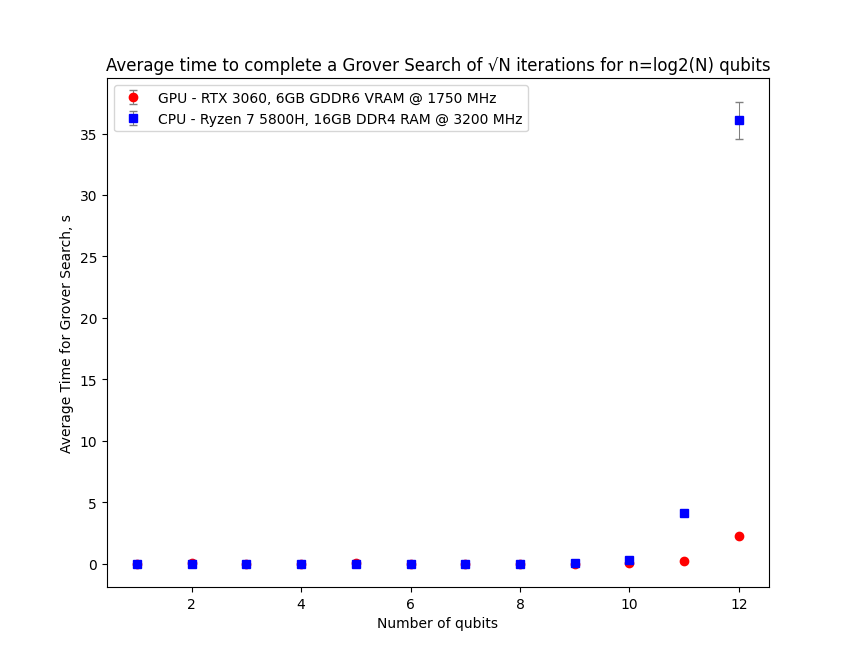
\includegraphics[width=\textwidth]{Pictures/CPU vs GPU full.png}
\caption{Average time taken to simulate Grover search with $n$ qubits on an $N=2^n$ element database for both the CPU and GPU versions of the simulation, as measured over 10 shots. Measurements were taken on a laptop with a Nvidia RTX 3060 GPU (6GB GDDR6 VRAM) and an AMD Ryzen 7 5800H CPU (16GB DDR4 RAM). For low qubit counts the performance difference is negligible, however around 9-10 qubits the computation time on the CPU grows exponentially faster than on the GPU.}
\label{fig:GPU_graph}
\end{figure}
It can be seen in Figure \ref{fig:GPU_graph} that the performance of the simulation does not differ greatly between the CPU and GPU versions for low qubit counts. However, once the qubit count becomes large enough the GPU version of the simulation is exponentially more performant than the CPU version.

That said, as with the CPU version the qubit count of the GPU simulation is limited by the capacity of the GPU's VRAM. With the computer available to us we were limited to $n=14$ qubits in the GPU version, the same amount we were limited to in the CPU version. In order to go beyond 14 qubits efficiently both versions would require making use of sparse matrix computing libraries. This would mean the full matrices are not stored in memory but are instead stored in a more optimised format, allowing for larger matrices to be used in the computations.\cite{candela} Even so, there is only so far this can take us as any simulated quantum computer will ultimately not be as performant as its physical analogue.

\pagebreak
\section{Shor's Algorithm and the RSA Cryptosystem}
\subsection{RSA Encryption/Decryption Algorithm}
The RSA (\textit{Rivest–Shamir–Adleman}) cryptosystem algorithm is a form of public-key encryption that is widely used to secure data transmission over the internet. This algorithm uses two keys, a \textit{public key} and a \textit{private key}, to encrypt and decrypt data.\cite{RSA} The public key is freely available to anyone who wants to send a message to the owner of the private key, while the private key is kept secret and only known to the owner. To encrypt a message using RSA, the sender uses the recipient's public key to convert the message into an unintelligible form that can only be decrypted using the recipient's private key. To decrypt the message, the recipient uses their private key to reverse the process and recover the original message. This algorithm consists of three stages:\cite{RSA}
\begin{itemize}
  \item Key generation.
  \item Key distribution
  \item Encryption (and decryption)
\end{itemize}

First, two large random prime numbers $p$ and $q$ of similar magnitude are produced such that their product is a composite number $N$. The \textit{Euler Totient} of $N$
\begin{equation}
\phi(N)=(p-1)(q-1)
\end{equation}
is then calculated, which is used to compute the public and private keys and is kept secret. A number $2<e<\phi(N)$ is then chosen such that $\text{gcd}(e,\phi(N))=1$. For the implementation in this report, $e$ is chosen at random with this constraint, however in practice there are standards for good choices of $e$.\cite{RSAattack} The pair $(e,N)$ is then publicised as the \emph{public key}.\cite{RSA} For the private key, we compute a number \\$d=e^{-1}\mod\phi(N)$ (i.e. a number $d$ such that $ed=1\mod\phi(N)$). The pair $(d,N)$ is the \emph{private key} and is known only to the recipient of any encrypted messages.\cite{RSA}

Imagine we have two people, Alice and Bob. If Bob wants to send information privately to Alice, Bob must know Alice's public key to encrypt the message, and Alice must use her private key to decrypt the message. Alice’s private key is never distributed, unlike her public key. For the encryption code, each character $m$ (stored as a binary number in some format such as unicode) is converted to a new character $c$ via the formula $c=m^e\mod N$ to form the ciphertext.\cite{RSA} For the decryption code, each element of the ciphertext is converted back to the original character $m$ via the equation $m=c^d\mod N$.\cite{RSA}

For the implementation of RSA in this project, $N$ was restricted to having a minimum length of 8 bits. The number of bits could be varied, however the 8-bit implementation of RSA is what was almost exclusively used in all applications.
\begin{figure}[H]
    \centering
    \begin{tabular}{||c|c|c|c|c|c|c||}
        \hline
        N & e & d & Plaintext & Plaintext Unicode & Ciphertext & Ciphertext Unicode \\
        \hline
        221 & 19 & 91 & ``hello'' & 104,101,108,108,111 & ``ÃeÇÇ '' & 195,101,199,199,32 \\
        \hline
        247 & 157 & 205 & ``world'' & 119,111,114,108,100 & ``]°rºJ'' & 93,176,114,186,74 \\
        \hline
    \end{tabular}
    \caption{Example public, private key pairs and the corresponding ciphertext for some sample messages. For both of these examples $N$ is an 8-bit integer, meaning this is an example of 8-bit RSA encryption.}
    \label{fig:RSA_example_table}
\end{figure}

In order to find the private key from the public key, it is necessary to factorise $N$ into the original prime numbers $p,q$ so that $\phi(N)$ can then be computed (and hence $d$, the private key).\cite{RSA} However, factorising a very large $N$ is currently considered an intractable problem for classical computers.\cite{nielsenChuang,RSAattack} As a result, RSA encryption is considered to be very secure against classical computers. 

On the other hand, it turns out that it is \emph{not} secure against quantum computers due to the existence of Shor's Algorithm, a quantum algorithm that can factorise integers much faster than any classical algorithm.

\subsection{Shor's Algorithm}\label{section:shor}
Given the composite number $N$, Shor’s algorithm can be used to find its prime factors $p$ and $q$ very quickly. It relies on a key fact: for any pair of integers $a, N$ that do not share any factors, it is always possible to find some $r\in\mathbbm N$ such that:\cite{nielsenChuang,Shors_algorithm}
\begin{equation}
a^r=\lambda N+1
\end{equation}
where $\lambda N$ is just some multiple of $N$. Assuming $r$ is even, we can then rearrange this equation as $(a^{r/2}+1)(a^{r/2}-1)=\lambda N$. This equation is clearly just a statement that $\lambda N$ can be written as the product of two numbers. This means we now have a factorisation formula! We simply compute $a^{r/2}\pm 1$ and then compute the greatest common divisor between this number and $N$ to find the factors of $N$, i.e.:\cite{candela,shorcircuit}
\begin{equation}
N=pq \Rightarrow (p,q)=\left(\gcd(a^{r/2}+1,N),\gcd(a^{r/2}-1,N)\right)
\end{equation}

Shor's algorithm therefore works to factorise $N=pq$ as follows:
\begin{enumerate}
    \item Generate a random number $1<a<N$
    \item If $\gcd (a,N)\neq 1$ (i.e. they share factors), then the algorithm is already done as $p=gcd(a, N)$ and $q=\frac{N}{p}$. This is because the only factors of $N$ are $p$ and $q$.
    \item Otherwise, find the value of the period $r$
    \item Computer the pair $\left(\gcd(a^{r/2}+1,N),\gcd(a^{r/2}-1,N)\right)$. These will be the prime factors of $N$
\end{enumerate}

The problem that therefore needs to be solved is finding the period. On a classical computer this could take a prohibitively long amount of time as it will have to search every even number one-by-one until it finds a value that works. This is where quantum computing comes in, as we can use a ``quantum period-finding subroutine'' to compute $r$ instead.

\subsubsection{The Quantum Period-Finding Subroutine}
This quantum part of Shor's algorithm is centered around a series of ``modular exponentiation'' quantum gates $\hat U_k$ that satisfy:\cite{shorcircuit}
\begin{equation}
\hat U_k\ket{x,y}=\ket{x,k^xy\hspace{-0.3cm}\mod N}
\end{equation}
These gates require two qubit registers, one for $x$ and one for $y$. If $N$ is an $M$-bit integer this means the $y$-register (known as the ancillary register) must have $M$ qubits, however the $x$-register (known as the main/working register) may have any number $L$ of qubits.

We first initialise the ancillary register into the state $\ket{1}$ (i.e. for a 4-bit ancillary register, this would be $\ket{0001}$).\cite{Shors_algorithm,candela} For each qubit of index $x$ in the main register, the gate $U_{a^{2^x}}$ is then applied to the ancillary register in such a way that the main qubit becomes entangled with the ancillary qubits. By placing the working register into a state where every input is equally likely, we can check all possible inputs \emph{simultaneously}. Once this is done, the ancillary register is then measured.\cite{candela} Due to the entanglement, this results in a probability distribution in the main register with peaks separated by $r$ (i.e. the distribution will be periodic with frequency of $r$). This can be converted into peaks at $r$ and multiples thereof using an inverse Fourier transform, which can be directly implemented in a quantum computer by passing the working qubits through a dedicated quantum inverse fourier transform circuit.\cite{candela,shorcircuit,Shors_algorithm}

\begin{figure}[H]
    \centering
    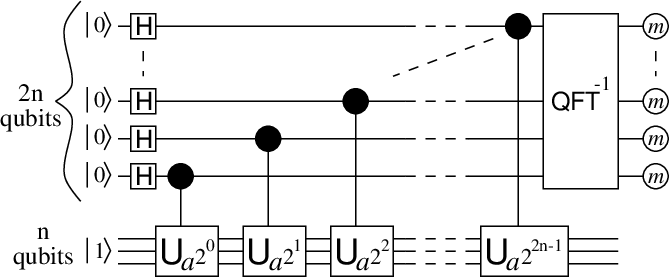
\includegraphics[width=0.6\textwidth]{Pictures/Shor's Circuit Diagram.png}
    \caption{The circuit diagram for the quantum part of Shor's algorithm. By passing the main register through a set of Hadamard gates, every possible input can be tested simultaneously instead of going through each of them one-by-one. The number of qubits in the main/working register does not strictly have to be $2n$, but as a general rule of thumb $2n$ is a good amount to use.\cite{candela} Figure taken from Beauregard - \emph{Circuit for Shor's algorithm using 2n+3 qubits.}\cite{shorcircuit}}
    \label{fig:shor_circuit}
\end{figure}

\subsubsection{Modular Exponentiation}
The quantum circuit diagram for the period finding part of Shor's algorithm is shown in Figure \ref{fig:shor_circuit}. The first section of this circuit consists of controlled-$U$ gates\footnote{See Appendix \ref{appendix:tablegates}}, which can be constructed via the following algorithm:\cite{candela}
\begin{enumerate}
    \item Begin by constructing a square empty matrix of size $2^{L+M}$, where $L$ is the number of working qubits and $M$ is the number of ancillary qubits.
    \item For each column in this matrix, write out the column number $c$ as a binary number: $(l_{L}...l_{0}m_{M}...m_{0})$.
    \item For a $U$ matrix controlled by a main register qubit $x$, the respective value of the binary number $l_x$ must be checked. If $l_x=0$ then set the entry on row $c$ equal to 1, similar to the identity matrix. The point being that if $l_x=0$ then nothing is done to the ancillary register.
    \item If $l_x=1$ then check the value of the binary number $b=(m_{M}...m_{0})$. If the value of this number $b$ is greater than or equal to the number to be factored, $N$, then then set the entry on row $c$ equal to 1 again.
    \item If $l_x=1$ and $b<N$, compute $b' = A_x\hspace{-0.1cm}\mod N$ where $A_x = a^{2^x}$. This new number is then written in binary form: $(b'_{M}...b'_{0})$. The entry equal to a 1 instead of a 0 is then located on row $j$, where $j=(l_{L}...l_{0}b'_{M}...b'_{0})$. The idea here is that if $m_x=1$, the ancillary register is multiplied by $A_x\hspace{-0.1cm}\mod N$.
    \item This is repeated for all main register qubits, generating the $U_{a^{2^x}}$ gates shown in Figure \ref{fig:shor_circuit}.
\end{enumerate}

\subsubsection{Inverse Quantum Fourier Transform}
Once the controlled-$U$ gates are applied, the ancillary register is measured and discarded to produce a probability distribution in the main register with frequencies close to multiples of $r$. As mentioned earlier, these frequencies can be converted into a peak at $r$ and multiples thereof by applying an inverse quantum fourier transform (IQFT) to the main register. The QFT is implemented in a quantum computer using the circuit in Figure \ref{fig:IQFT}.\cite{nielsenChuang}
\begin{figure}[H]
    \centering
    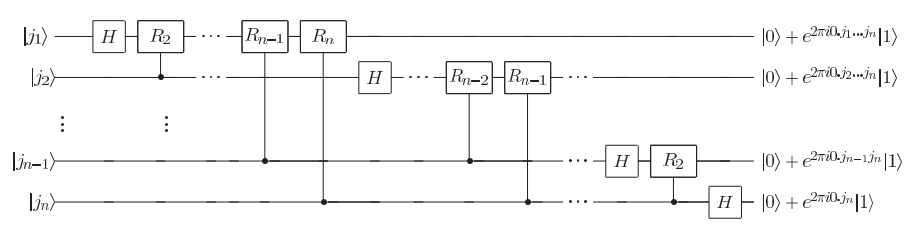
\includegraphics[width=0.85\textwidth]{Pictures/qft_nc.png}
    \caption{Circuit diagram of the quantum fourier transform. Note that whilst the first qubit was on the bottom in Figure \ref{fig:shor_circuit}, it is located on the top here. Figure taken from Nielsen and Chuang.\cite{nielsenChuang}}
    \label{fig:IQFT}
\end{figure}

The controlled gates $R_n$ are known as ``controlled rotation'' gates (CROT) and they are defined as:\cite{nielsenChuang}
\begin{equation}
R_n=\begin{pmatrix}
1&0&0&0\\
0&1&0&0\\
0&0&1&0\\
0&0&0&e^{\frac{2 \pi i}{n}}
\end{pmatrix}
\end{equation}

To turn this into an \emph{inverse} quantum fourier transform, the sign in the exponential is flipped (i.e. $e^{-2\pi i/n}$ instead of $e^{2\pi i/n}$). Once the IQFT is applied the resulting probability distribution in the main register will have peaks close to multiples of $\frac{2^L}{r}$, where $r$ is the period and $L$ is the number of working qubits. As a result, the working register can now be measured at this point. The resulting bitstring is divided by $2^L$ to find a value we shall call the \emph{``phase.''} This phase will be close to a multiple of $\frac{1}{r}$ and is then finally used to estimate the period using a continued fraction expansion.\cite{candela}

\subsubsection{Estimating the period}
The value of the phase $\frac{y}{Q}$ should be close to a multiple of $\frac{1}{r}$, where $r$ is the true period. If we are lucky this equality is exact, but otherwise we must estimate the period. To do this, we expand $\frac{y}{Q}$ into a continued fraction:
\begin{equation}
\frac{y}{Q}=a_0+\frac{1}{a_1+\frac{1}{a_2+\frac{1}{\dots+\frac{1}{a_n}}}}
\end{equation}
By terminating the expansion early, we are able to compute a series of approximations $\frac{s}{p}\approx\frac{y}{Q}$. We can then search through multiples of the denominators of these approximations, $\lambda p$, until one is found that satisfies the condition $a^{\lambda p} = 1\mod{N}$. This is then the estimated period $r$ and the factors are computed as $\gcd(a^{\frac{r}{2}}\pm 1,N)$.


\subsection{Results}
\subsubsection{Implementation of Shor's Algorithm}
Using the simulation methods described in section \ref{section:simulation}, Shor's algorithm was implemented to (in principle) factorise \emph{any} given integer. However, in practice the hardware limitations of the simulation (13 qubits) meant that we could at most implement the algorithm for factorising integers described by a small number of bits.

For the first test, Shor's algorithm was applied to the task of factorising $N=15$ (a 4-bit integer). The size of the working register was varied between 3 to 6 qubits\footnote{Including the ancillary reigster, this means the total number of qubits was varied between 7 and 10 qubits} and the pivot was fixed to $a=7$ for consistency. At this point, no error simulation as outlined in section \ref{section:error_intro} was included.
\begin{figure}[H]
\centering
\begin{subfigure}[t]{0.5\textwidth}
\centering
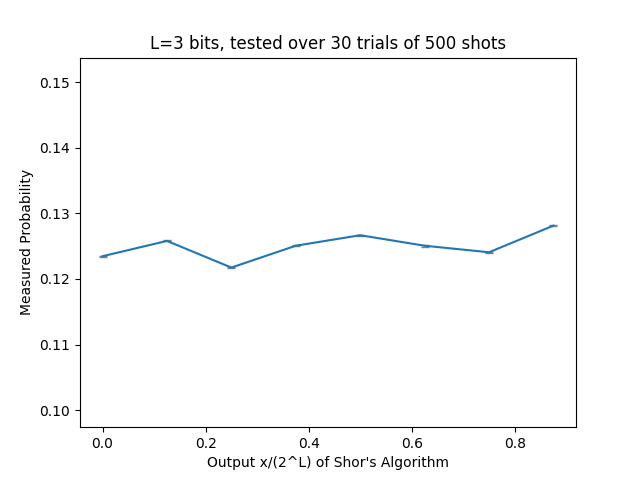
\includegraphics[width=\linewidth]{Pictures/Shor Factor 15/shor 3 bits factor 15 errorp 0.png}
\end{subfigure}%
\begin{subfigure}[t]{0.5\textwidth}
\centering
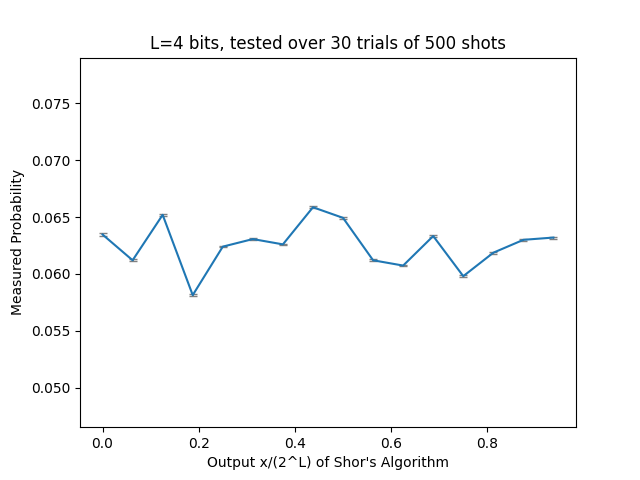
\includegraphics[width=\linewidth]{Pictures/Shor Factor 15/shor 4 bits factor 15 errorp 0.png}
\end{subfigure}
\begin{subfigure}[t]{0.5\textwidth}
\centering
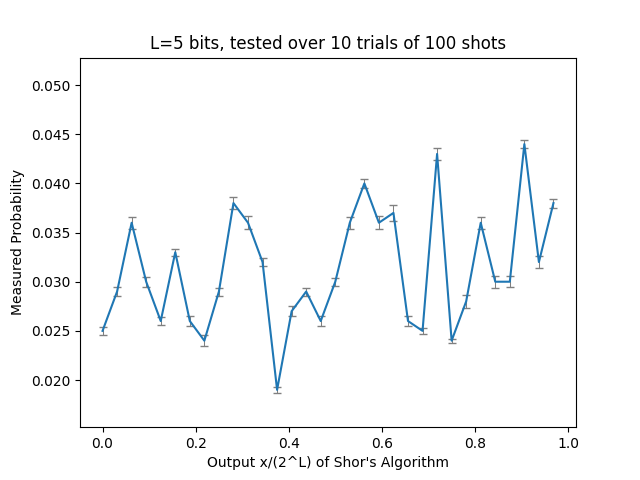
\includegraphics[width=\linewidth]{Pictures/Shor Factor 15/shor 5 bits factor 15.png}
\end{subfigure}%
\begin{subfigure}[t]{0.5\textwidth}
\centering
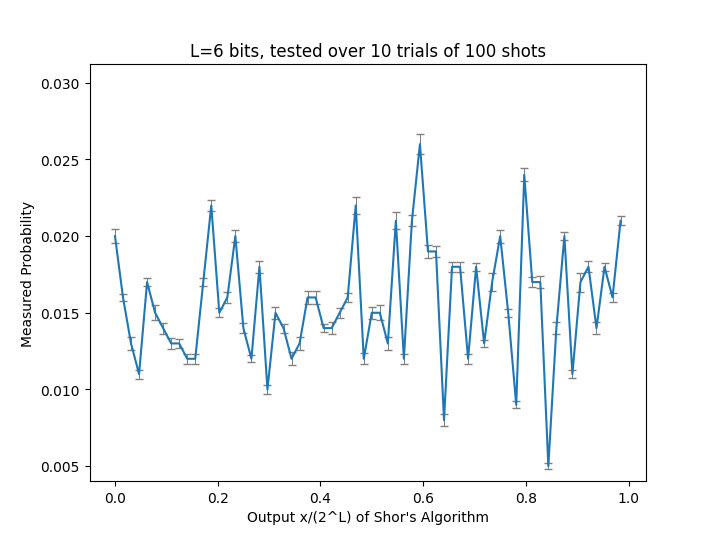
\includegraphics[width=\linewidth]{Pictures/Shor Factor 15/shor 6 bits factor 15.png}
\end{subfigure}
\caption{Measured probability distributions for the output of the quantum period-finding subroutine circuit for factorising $N=15$ using different sizes $L$ of the working register, using a fixed pivot of $a=7$. As the number of qubits increases the local peaks become more frequent and well-defined, meaning the probability of a successful factorisation increases.}
\label{fig:factor15}
\end{figure}

Figure \ref{fig:factor15} demonstrates that as the number of qubits increases, the local peaks in the probability distribution become more frequent and more sharply defined. This is as expected, since the algorithm will have a greater degree of precision in finding a value close to $\frac{1}{r}$ and multiples thereof. It should be noted that these are not global peaks and the probability of measuring a specific peak is quite low, but Shor's algorithm only requires that any of the peaks is the outcome to find $r$. Overall this implies that as the number of qubits in the working register increases, the probability of a successful factorisation also increases.

With this in mind, the probability of a successful factorisation of $N=15$ as the number of working qubits varied was then experimentally measured. It was also measured for $N=39$ as well. Barring one outlier, these measurements confirmed that an increase in qubits led to an increase in successful factorisations.
\begin{figure}[H]
    \centering
\begin{subfigure}[t]{0.48\textwidth}
    \centering
    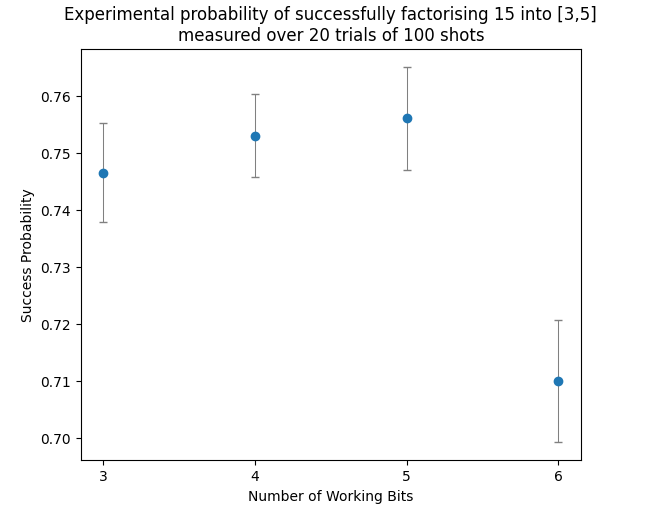
\includegraphics[width=\linewidth]{Pictures/Shor Factor 15/shor factor 15 bitsize test.png}
\end{subfigure}%
\begin{subfigure}[t]{0.52\textwidth}
    \centering
    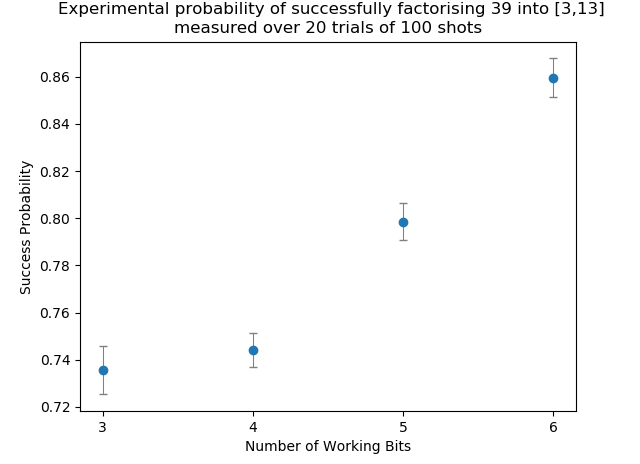
\includegraphics[width=\linewidth]{Pictures/Shor Factor 15/shor_39_factor_graph.png}
\end{subfigure}
\caption{The experimentally measured probabilities of Shor's algorithm successfully factorising 15 and 39 for various sizes $L$ of the working register. Generally speaking there appears to be an increase in the probability of success as the working register grows, as expected. However, there is an outlier: there is roughly a 4\% drop in the success rate for $N=15$ when $L=6$. We believe this is likely just sampling bias (since there were only 20 trials), but further investigation would be required to prove or disprove this.}
\label{fig:factortest}
\end{figure}

Figure \ref{fig:factortest} demonstrates that even for relatively small qubit counts the odds of Shor's algorithm successfully factorising an integer are quite good (at least 75\%). Shor's algorithm was therefore applied to the task of breaking \emph{8-bit RSA encryption}. Given a randomised public key $(e,N)$, Shor's algorithm was used to factorise $N$ (an 8-bit integer). This was used to compute guesses for $\phi(N)$ and then $d$, the private key. This guess for $d$ was then compared to the true private key and it was recorded whether the guessed key was correct or incorrect. The overall probability of success was then measured for different sizes of the working register.

\begin{figure}[H]
    \centering
    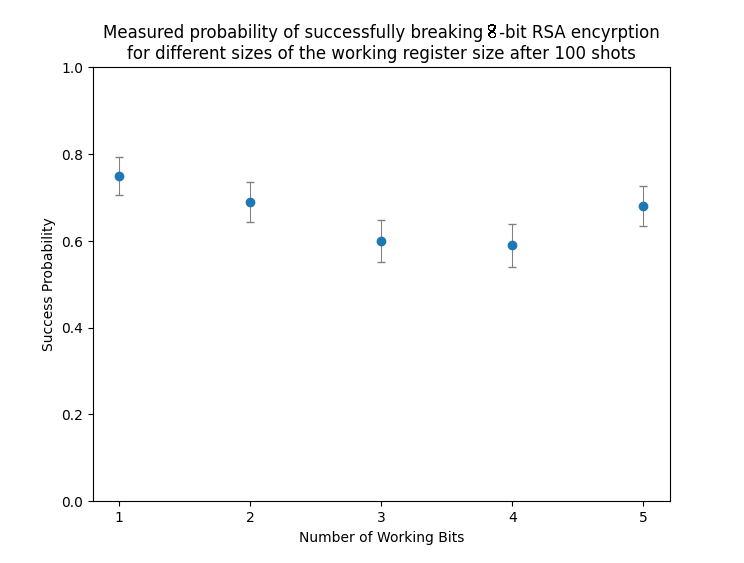
\includegraphics[width=0.8\textwidth]{Pictures/RSA Breaking/rsa_cracking_alt.png}
    \caption{The probability of successfully breaking 8-bit RSA encryption (i.e. finding the private key from the public key) for different working register sizes. Overall the probability of success is around 60-75\% for this range of working register sizes. Due to previously mentioned hardware limitations we are limited to 13 simulated qubits overall. This means the working register of 5 qubits is a hard limit, since there will always be 8 ancillary qubits.}
    \label{fig:RSA_cracking}
\end{figure}

Figure \ref{fig:RSA_cracking} demonstrates that it is indeed possible for Shor's algorithm to break RSA encryption. However, for the working register sizes chosen here the probability of success if not necessarily ideal (only 60-75\%). This is because factorising an 8-bit integer would ideally require a working register of between 11 to 17 qubits.\cite{candela,shorcircuit} Unfortunately this was beyond the abilities for our simulation as we were limited to a total of just 13 qubits. Since an 8-qubit ancillary register was already required, this means the largest working register we could use here was $L=5$.

\subsubsection{Error Simulation}\label{section:errorshor}
Having now considered a noise-free implementation of Shor's algorithm, we now consider the implementation of Shor's algorithm \emph{with} randomised computational error using the method in Section \ref{section:error_intro}. Whilst Grover Adaptive Search was previously shown to be quite stable against such errors as expected, it was less clear how Shor's algorithm would be affected by such errors.

For the first test, the noisy version of Shor's algorithm was tasked with factorising $N=15$ using working registers of 3 and 4 qubits. The probability of errors $p_e$ and the error size $\Omega$ were both varied to test how an increase in noise levels would affect the outcome. The algorithm was run multiple times and each time it was recorded whether the factorisation was successful or not.
\begin{figure}[H]
\centering
\begin{subfigure}[t]{0.65\textwidth}
\centering
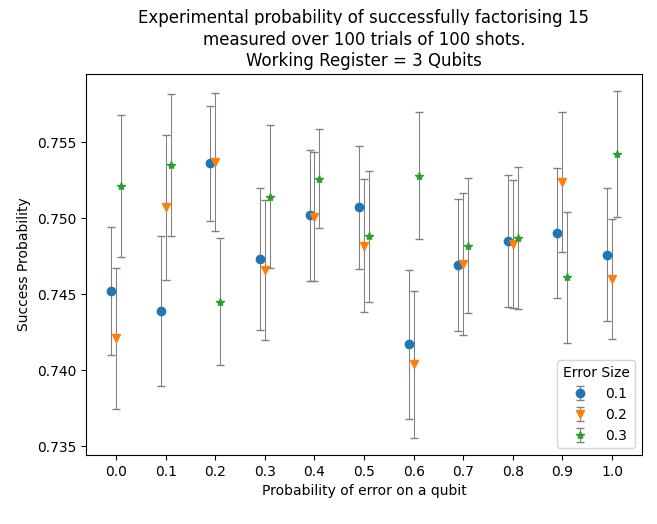
\includegraphics[width=\linewidth]{Pictures/Shor Factor 15/factor 15 error test.png}
\end{subfigure}
\begin{subfigure}[t]{0.65\textwidth}
\centering
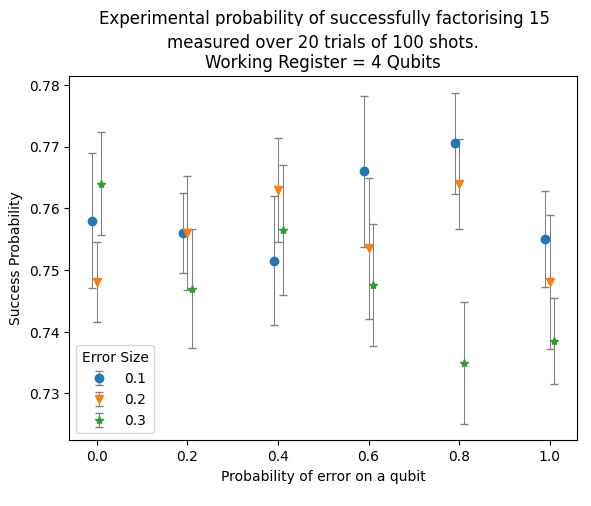
\includegraphics[width=\linewidth]{Pictures/Shor Factor 15/factor 15 error test 2.png}
\end{subfigure}
\caption{The measured probability of successfully factorising 15 into its non-trivial factors (5 and 3) for different values of the error probability. Working registers of $L=3,4$ qubits and error sizes of $\Omega=0.1,0.2,0.3$ were tested. Overall the success rate seems relatively stable at around 75\%. Whilst lower than ideal, this is still quite effective for such small working registers.}
\label{fig:factor15errors}
\end{figure}

Figure \ref{fig:factor15errors} shows that overall Shor's algorithm was not greatly impacted by the introduction of random error when factorising $N=15$, with the success probability only differing marginally as the amount of noise changed. The effect was slightly more noticeable for a larger error size of $\Omega=0.3$, but was still quite small.

The impact of random error was then tested for the application of Shor's algorithm to breaking RSA encryption.

\begin{figure}[H]
\centering
\begin{subfigure}[t]{0.7\textwidth}
\centering
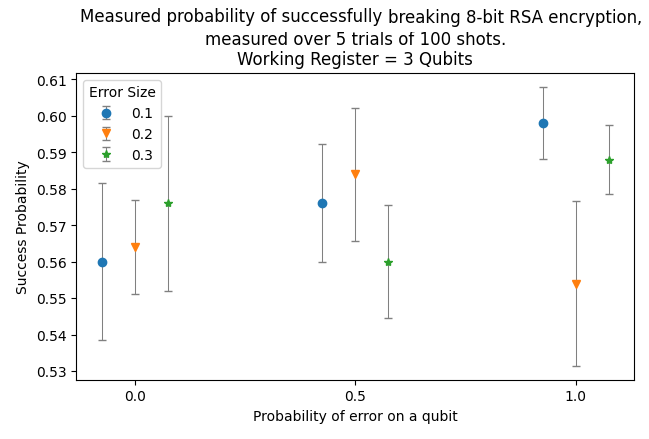
\includegraphics[width=\linewidth]{Pictures/RSA Breaking/rsa break errorp test 3 qubits.png}
\end{subfigure}
\begin{subfigure}[t]{0.7\textwidth}
\centering
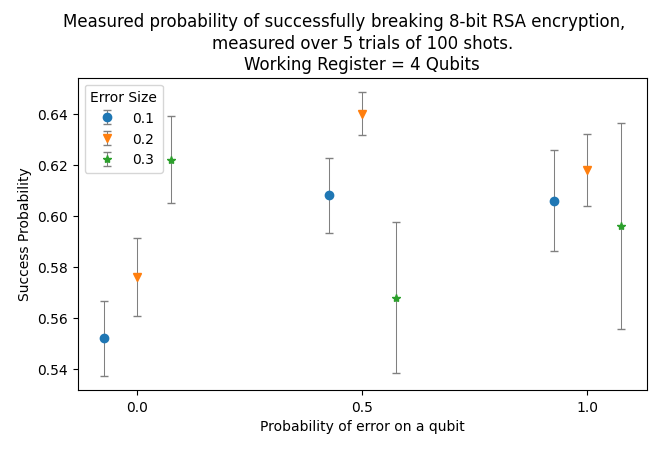
\includegraphics[width=\linewidth]{Pictures/RSA Breaking/rsa break errorp test 4 qubits.png}
\end{subfigure}
\caption{The measured probability of successfully breaking 8-bit RSA encryption (i.e. finding the private key from the public key) using Shor's Algorithm for different values of the error probability. Working registers of $L=3,4$ qubits and error sizes of $\Omega=0.1,0.2,0.3$ were tested. As also observed when factorising $N=15$, the success rate is generally stable with respect to the errors. The overall average success rate is not very high for these working register sizes (roughly around 55-60\%), however this is as expected as such working registers are small compared to the 8-bits used in the RSA encryption.}
\label{fig:breakRSAerrors}
\end{figure}

Again, Figure \ref{fig:breakRSAerrors} demonstrates that Shor's Algorithm remains relatively stable for breaking 8-bit RSA encryption even when under the influence of random error. The overall probabilities of success are not generally high (around 55-60\%), but this is consistent with the results seen earlier without any error simulation and is an artifact of the small working register. It should be noted that the variation is slightly larger here than it was for factorising $N=15$, however it is important to note the number of trials was much lower and hence the data will be less precise. Overall the variation is still quite small. It may be the case that a larger working register would be more greatly impacted. Testing this was not possible for us to do however, as the simulation was already near the limits of what could be achieved with the hardware available to us. 

\subsubsection{A Classical Version of Shor's Algorithm}
As discussed in Section \ref{section:shor}, the only part of Shor's Algorithm which actually makes use of quantum computing is the quantum period-finding algorithm; the rest is completely classical.\cite{candela} This indicates that it is also technically possible to implement a completely classical version of Shor's Algorithm where this quantum algorithm is replaced with just a classical linear search. This means searching through every number between $1$ and $N-1$ for a number $r$ that satisfies:
\begin{equation}
    a^r\hspace{-0.3cm}\mod N=1
\end{equation}

Using this classical linear search for Shor's Algorithm, a large number of different randomised semiprimes were factorised and the time taken for each factorisation was measured. Each of these semiprimes were classified by the minimum number of qubits a quantum implementation would require to factorise them. For any integer $N$, the number of bits required to represent it is $\lceil\log_2N\rceil$. This means that the minimum number of qubits Shor's Algorithm needs to factorise $N$ with a high probability of success is\cite{candela} $q=\lfloor1+2\log_2N\rfloor$.
\begin{figure}[H]
\centering
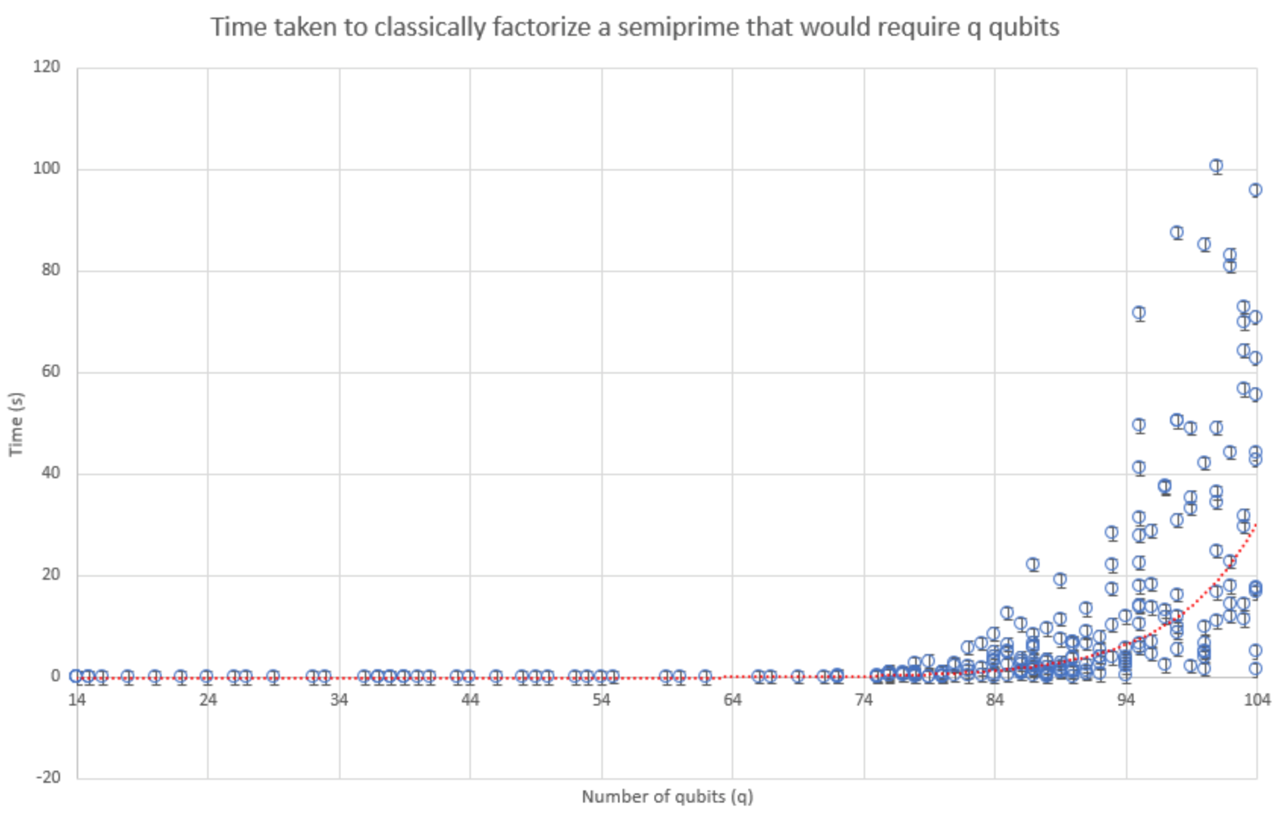
\includegraphics[width=\textwidth]{Pictures/Time taken to classically factorize a semiprime that would require q qubits Large.png}
\caption{Graph of the classical factorisation algorithm runtime against the number of qubits $q$ that would be required \emph{if} one were to factorize the same semiprime integer $N$ using the quantum algorithm. Different semiprimes were factorised and they were grouped by their corresponding $q$ values. An exponential curve of best fit (red dotted line) lies on top of the data.}
\label{fig:Classical factorization graph}
\end{figure}

It can be seen in Figure \ref{fig:Classical factorization graph} that the measured runtime is close to $0$ seconds for semiprimes that would require $75$ qubits, and then the exponential nature of this classical algorithm begins to become apparent. This makes sense, since if the number of bits to represent $N$ increases by 1 then total number of possible values for $r$ that must be checked will double. This means the theoretical time complexity of finding the period for factorising an $m$-bit integer with this algorithm is at least $O(2^m)$ (not including the time complexity required to compute $a^r\hspace{-0.2cm}\mod N$).

However, there is deviation from the exponential model as the algorithm picks random values for the pivot $a$. This means the number of values the algorithm must search through to find the period $r$ will not be consistent and hence the variation of run-times becomes larger with $q$ (since there are more value of $a$ to choose). There is also always the chance of the pivot $a$ being a factor of $N$ itself as well, which would lead to to the search not being run at all. This chance is $\frac{2}{N-1}$, which vanishes as $N$ tends to infinity. Still, it is clear that overall this data demonstrates that the runtime for such a classical algorithm grows exponentially. %this might be good to onclude in the further work section?


\pagebreak
\section{Conclusions}
\subsection{Unstructured Search and Quantum Algorithms}
Using quantum algorithms such as Grover's Algorithm and GAS for unstructured search on large databases can offer notable advantages over classical algorithms, since they provide significant speedups on time complexity.\cite{grover,baritompa} This can lead to remarkable time savings in applications that require searching through very large databases, such as financial analysis, natural language processing and even genomics search.\\
\\
However, implementing such  algorithms on classical computers comes with significant drawbacks. The performance of quantum algorithms is greatly limited by the resources available on classical computers, as the number of possible states for a given number of qubits vastly exceeds the number of states for the same number of classical bits. As we have seen in this report, this means we can only do so much with a classical computer. Although we have shown that GAS works perfectly, the computational resources it requires are significant and overall it is clear that \textbf{when using a classical computer it is still more useful to implement classical algorithms.} Classical computers do not intrinsically have the necessary \textit{``quantumness''} for these algorithms, which require quantum mechanical properties such as superposition, entanglement, and interference.\cite{nielsenChuang} Thus simulating quantum algorithms on classical computers requires significant computational resources and ideally specialist hardware like GPUs, which limits the size of the problems that can be addressed.\\
\\
In summary, the challenges associated with implementing these algorithms on classical computers are significant, and the full potential of quantum computing can only be properly realised on actual quantum computers. Our simulations do however suggest that they are immensely performant as predicted, requiring less quantum gate computations to perform compared to their classical counterparts. Once actual quantum computers progress far enough in their development the full advantages of these algorithms will become much more apparent.

\subsection{Security}
Overall, it is clear that it is very possible for Shor's Algorithm to break RSA encryption. Even given the hardware limitations of the simulation discussed in this project, it was still 60\% successful at breaking 8-bit RSA encryption, which in practice means the algorithm would only have to be run once or twice. Given a larger number of working qubits this success rate would likely increase, since Shor's algorithm is more likely to output the correct period $r$ as the working register grows.\cite{candela}\\
\\
RSA's severe vulnerability to Shor's algorithm is quite dangerous, since RSA encryption is a very widely used cryptosystem due to its high security against classical computers.\cite{RSAattack} However, typical modern RSA keys are 1024 to 4096 bits in length.\cite{nist} Assuming a working register of equal size to the ancillary, this would mean 2048 to 8192 qubits would be required to break any actual form of RSA encryption.\cite{candela,shorcircuit} This is beyond the capabilities of current quantum computers, so RSA encryption is still deemed a safe cryptosystem for the time being. However, in the future this will not be the case once quantum computers develop further and will necessitate using either ``quantum-safe'' classical cryptosystems or fully quantum cryptosystems.\\
\\
For example, AES-256 (which generates 256 bit keys) is a classical cryptosystem which is deemed quantum-safe.\cite{ETSI_threat_assess} It is symmetric, meaning that no two different keys are produced, and the key produced is kept secret between the sender and the receiver. Grover's Algorithm could potentially be used as an attack vector against such a problem, but the required compute time is still enormous (since there are $2^{256}$ possible keys, the algorithm would need to perform $2^{128}$ iterations to search for the correct key).\cite{ETSI_threat_assess} \\
\\
Quantum cryptosystems can involve storing an encryption key as a qubit state.\cite{quantumcrypt} Such cryptosystems are then automatically quantum-safe by definition of the no-cloning theorem. The no-cloning theorem is a direct consequence of quantum mechanics, where it is impossible to create an identical copy of an unknown (unmeasured) pure quantum state. This is because the process of copying a qubit state onto a second qubit is fundamentally a non-unitary, irreversible transformation.\cite{nielsenChuang} The only way to ``eavesdrop'' would therefore be to measure the qubit state, which would automatically be detected as the state would collapse.\cite{quantumcrypt} Breaking a quantum cryptosystem using a classical computer would either be impossible or incredibly difficult, therefore the only threat to quantum cryptosystems is the (limited) potential of a quantum computer. Quantum-cryptosystems may also exploit entanglement-assisted quantum teleportation.\cite{quantumcrypt} This allows information about a quantum state to be transferred from one particle to another in a different location - this may be used as a means of quantum key distribution. However, quantum teleportation does involve the transfer of classical information between sender and receiver, thus quantum ``teleportation'' cannot happen faster than the speed of light. Moreover, quantum cryptosystems are unlikely to be accessible to all and so symmetric classical quantum-safe cryptosystems would need to suffice for most applications.

\subsection{Further work}
Although our simulations of both Grover's Adaptive Search Algorithm and Shor's Algorithm have provided insights into the behaviour of quantum systems and the performance of quantum algorithms, our computational resources were limited and thus there is still much more work that could be done.\\
\\
For example, in Section \ref{section:errorshor} we discussed how Figures \ref{fig:factor15errors} and \ref{fig:breakRSAerrors} present only a small variation in the overall probability of successful factorisations. We believe it is plausible that a larger register would be more greatly impacted. However, exploring the impact of larger working registers on our simulation was not possible for us to do due to hardware limitations. This could be explored in further projects on the subject by researchers who have access to greater computational resources. This can be said about most of the report, since more advanced hardware would have improved greatly the computation time (which is not to be confused with time complexity) of our algorithms, as well as allowing us to examine both of them with a larger number of qubits.\\
\\
Aside from using more powerful hardware, another more efficient means of simulating more than 14 qubits would be to make use of sparse matrix computing libraries. This would
mean the matrices are not stored in memory with all their components (many of which are empty) but are instead in a more optimised format, allowing for larger matrices to be used in the computations.\cite{candela} For a simulation in Python this could, for example, be implemented with the use of SciPy (and also CuPy).\cite{cupy2017,2020SciPy-NMeth}\\
\\
Furthermore, the error simulation itself could be further improved. The algorithm outlined in Section \ref{section:error_intro} simulates error via randomised $SU(2)$ matrices, which are then combined into $SU(2^n)$ matrices via tensor products. To be precise however, these matrices are actually elements of $SU(2)^{\otimes n}$, which is only a \emph{proper subset} of $SU(2^n)$.\cite{chenGroup} This difference is key as it means the error matrices are completely separable and thus cannot simulate error due to accidental entanglement of qubits. To simulate such entanglement error, it would be therefore necessary to implement non-separable $SU(2^n)$ matrices. This could be done, for example, by computing the generators of $SU(2^n)$ and then using these to construct the error matrices.



\pagebreak
\section{Acknowledgements}
This project has made use of data obtained from or tools provided by the portal exoplanet.eu of The Extrasolar Planets Encyclopaedia.

\bibliographystyle{unsrtnat}
\bibliography{refs}
\vspace{0.3cm}
All other figures, tables, etc. were created specifically for this report.


\pagebreak
\appendix
\section{Appendix}\label{section:appendix}
\subsection{Table of Quantum Logic Gates}\label{appendix:tablegates} 
\begin{figure}[H]
    \centering
    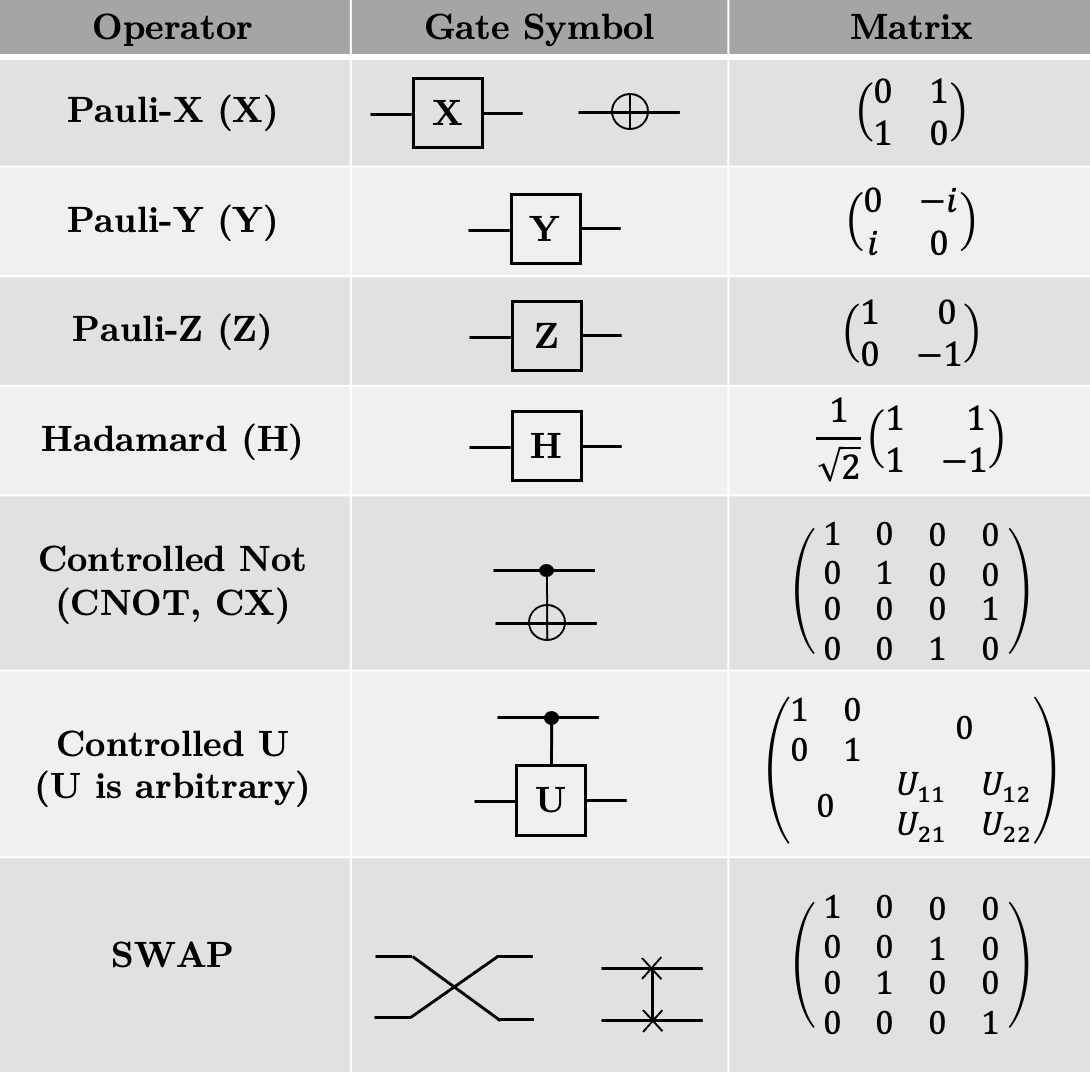
\includegraphics[width=\textwidth]{Pictures/quantumgates.png}
    \caption{A table of some commonly used quantum logic gates in quantum computers.\cite{nielsenChuang,candela,gate_table}}
    \label{fig:f}
\end{figure}


\pagebreak
\subsection{ESI Database}\label{appendix:ESI}
As discussed in section \ref{section:groverproject}, a database of exoplanets was extracted from The Extrasolar Planets Encyclopaedia to compute a database of planets that were quantified in habitability by their Earth Similarity Index. To recap, the ESI is a dimensionless parameter between 0 and 1 that is calculated using the following equation:
\begin{equation}
ESI_j=\prod^n_{i=1}{\left(1-\frac{x_{i,j}-x_{i,\bigoplus}}{x_{i,j}+x_{i,\bigoplus}}\right)^{w_i/n}}
\end{equation}
\begin{center}
\begin{tabular}{||c|c|c|c||}
\hline
$i$ & \textbf{Parameter} & \textbf{Earth value} $x_{i,\bigoplus}$ & \textbf{Weight} $w_i$ \\
\hline
1 & Radius  & 1.0  & 0.57 \\
\hline
2 & Density  & 1.0 & 1.07 \\
\hline
3 & Escape velocity  & 1.0 & 0.7 \\
\hline
4 & Surface temperature & 288K & 5.58 \\
\hline
\end{tabular}
\end{center} 

After collecting the data provided by the Extrasolar Planets Encyclopaedia\cite{EPE}, the database was trimmed to the subset of planets with a given mass, radius and temperature. The densities and escape velocities of each exoplanet were then calculated using their mass and radius (assuming that each planet was a perfect sphere). Finally, each exoplanet's ESI was computed. The calculations for the first 20 exoplanets are shown in the table below, where the mass and radius of each exoplanet are presented in units of Jupiter's mass and radius as used in the Extrasolar Planets Encyclopaedia.\cite{EPE}

 \tablehead{%
 \toprule
Name & Mass/$M_{Jup}$ & Radius/$R_{Jup}$ & Temperature/$K$ & ESI\tabularnewline
 \midrule}
 \tabletail{\midrule}
\tablelasttail{\bottomrule}
\begin{center}
\begin{supertabular}{||c|c|c|c|c||}
\csvreader[separator=semicolon, late after line=\\]{"trimmedagain.csv"}{1=\Name,2=\Mass,3=\Radius,4=\Temperature,5=\ESI}{\Name&\Mass&\Radius&\Temperature&\ESI}
 \bottomrule
 \end{supertabular}
 \end{center}


 \pagebreak
\subsection{Further Error Modelling Tests for the Durr-Hoyer Algorithm}\label{section:errorps}
\begin{figure}[H]
\centering
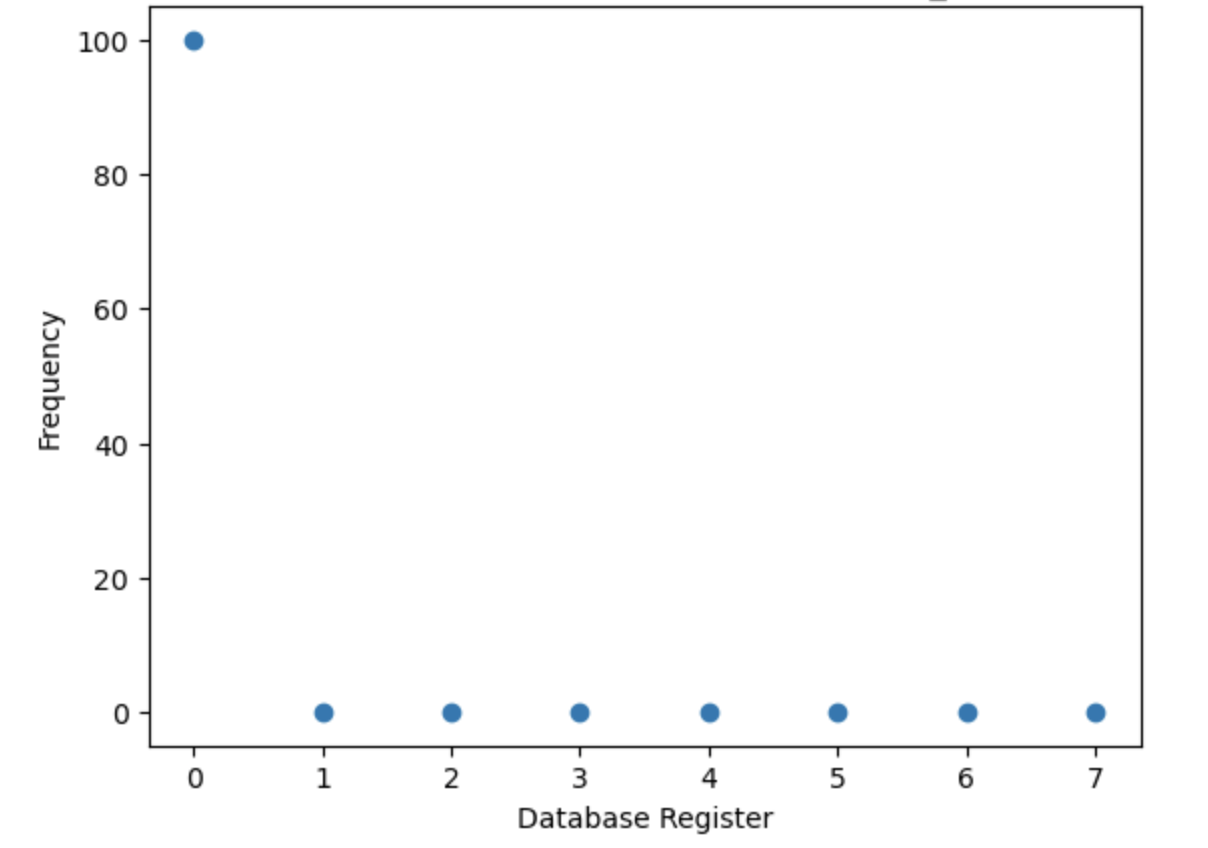
\includegraphics[width=0.6\textwidth]{Pictures/errorp03.png}
\caption{Frequency plot of the Durr-Hoyer algorithm when applied to a randomised 3-qubit database. Minimum value = 800. Error probability = 0.3.}
\label{fig:errorp03}
\end{figure}
\begin{figure}[H]
\centering
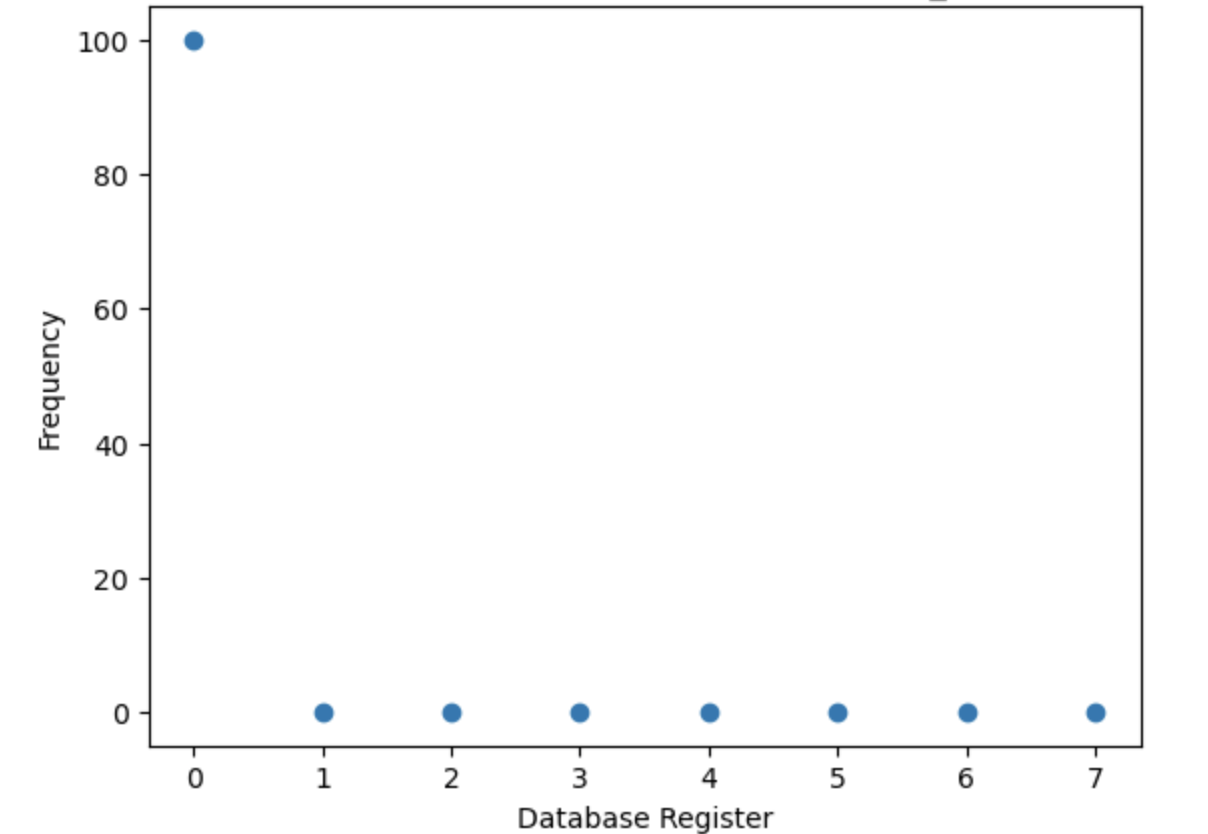
\includegraphics[width=0.6\textwidth]{Pictures/errorp05.png}
\caption{Frequency plot of the Durr-Hoyer algorithm when applied to a randomised 3-qubit database. Minimum value = 800. Error probability = 0.5.}
\label{fig:errorp05}
\end{figure}
\begin{figure}[H]
\centering
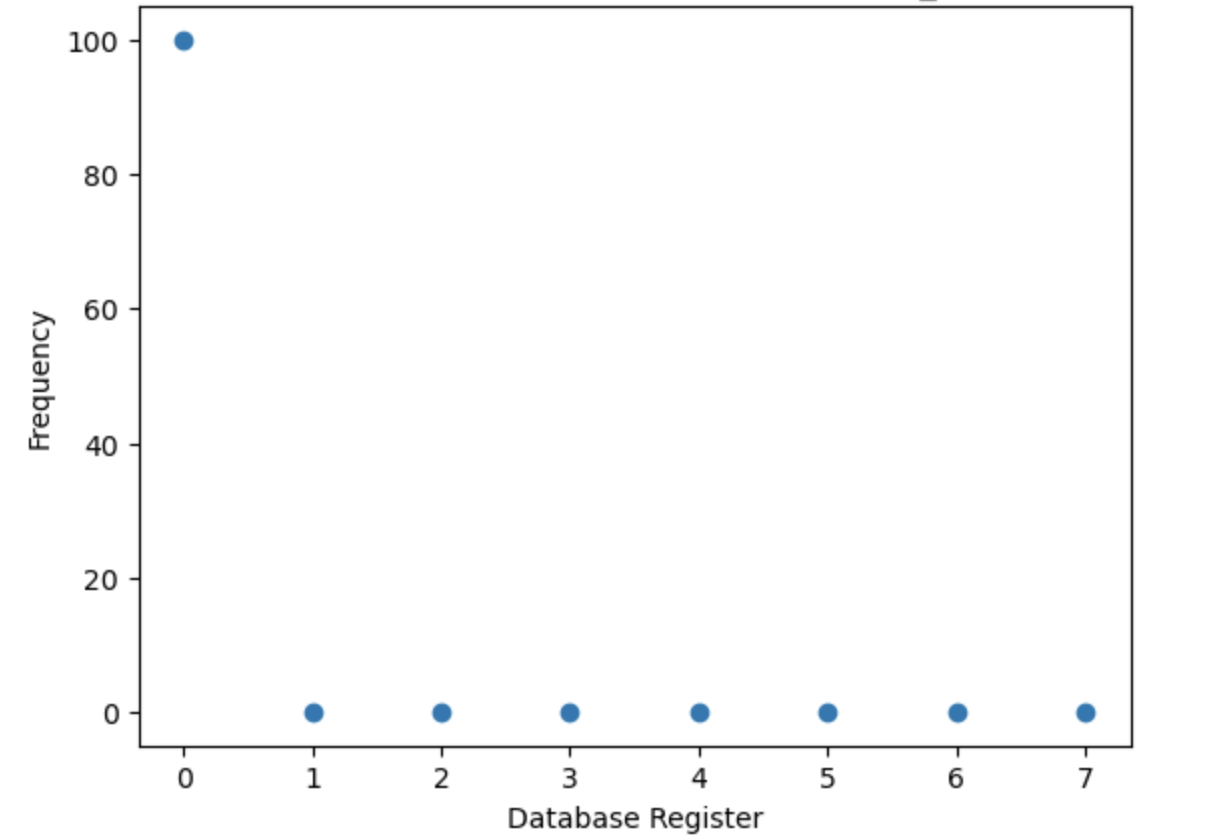
\includegraphics[width=0.6\textwidth]{Pictures/errorp07.png}
\caption{Frequency plot of the Durr-Hoyer algorithm when applied to a randomised 3-qubit database. Minimum value = 800. Error probability = 0.7.}
\label{fig:errorp07}
\end{figure}
\begin{figure}[H]
\centering
\begin{tabular}{||c|c||}
\hline
Error Probability & Runtime (seconds)\\
\hline
0 & 0.39375901222229004\\
0.1 & 0.42333078384399414\\
0.2 & 0.5374641418457031\\
0.3 & 0.6513032913208008\\
0.4 & 0.7484589862823486\\
0.5 & 0.8773360252380371\\
0.6 & 0.9940447807312012\\
0.7 & 1.0988891124725342\\
0.8 & 1.3646509647369385\\
0.9 & 1.5959539413452148\\
1 & 2.3649098873138428\\
\hline
\end{tabular}
\caption{Relationship between different error probabilities and time taken to run the simulation of the Durr-Hoyer algorithm for a 3-bit (8 element) database which is randomly generated.}
\end{figure}


\end{document}